% Options for packages loaded elsewhere
% Options for packages loaded elsewhere
\PassOptionsToPackage{unicode}{hyperref}
\PassOptionsToPackage{hyphens}{url}
\PassOptionsToPackage{dvipsnames,svgnames,x11names}{xcolor}
%
\documentclass[
  letterpaper,
  DIV=11,
  numbers=noendperiod]{scrreprt}
\usepackage{xcolor}
\usepackage{amsmath,amssymb}
\setcounter{secnumdepth}{5}
\usepackage{iftex}
\ifPDFTeX
  \usepackage[T1]{fontenc}
  \usepackage[utf8]{inputenc}
  \usepackage{textcomp} % provide euro and other symbols
\else % if luatex or xetex
  \usepackage{unicode-math} % this also loads fontspec
  \defaultfontfeatures{Scale=MatchLowercase}
  \defaultfontfeatures[\rmfamily]{Ligatures=TeX,Scale=1}
\fi
\usepackage{lmodern}
\ifPDFTeX\else
  % xetex/luatex font selection
\fi
% Use upquote if available, for straight quotes in verbatim environments
\IfFileExists{upquote.sty}{\usepackage{upquote}}{}
\IfFileExists{microtype.sty}{% use microtype if available
  \usepackage[]{microtype}
  \UseMicrotypeSet[protrusion]{basicmath} % disable protrusion for tt fonts
}{}
\makeatletter
\@ifundefined{KOMAClassName}{% if non-KOMA class
  \IfFileExists{parskip.sty}{%
    \usepackage{parskip}
  }{% else
    \setlength{\parindent}{0pt}
    \setlength{\parskip}{6pt plus 2pt minus 1pt}}
}{% if KOMA class
  \KOMAoptions{parskip=half}}
\makeatother
% Make \paragraph and \subparagraph free-standing
\makeatletter
\ifx\paragraph\undefined\else
  \let\oldparagraph\paragraph
  \renewcommand{\paragraph}{
    \@ifstar
      \xxxParagraphStar
      \xxxParagraphNoStar
  }
  \newcommand{\xxxParagraphStar}[1]{\oldparagraph*{#1}\mbox{}}
  \newcommand{\xxxParagraphNoStar}[1]{\oldparagraph{#1}\mbox{}}
\fi
\ifx\subparagraph\undefined\else
  \let\oldsubparagraph\subparagraph
  \renewcommand{\subparagraph}{
    \@ifstar
      \xxxSubParagraphStar
      \xxxSubParagraphNoStar
  }
  \newcommand{\xxxSubParagraphStar}[1]{\oldsubparagraph*{#1}\mbox{}}
  \newcommand{\xxxSubParagraphNoStar}[1]{\oldsubparagraph{#1}\mbox{}}
\fi
\makeatother

\usepackage{color}
\usepackage{fancyvrb}
\newcommand{\VerbBar}{|}
\newcommand{\VERB}{\Verb[commandchars=\\\{\}]}
\DefineVerbatimEnvironment{Highlighting}{Verbatim}{commandchars=\\\{\}}
% Add ',fontsize=\small' for more characters per line
\usepackage{framed}
\definecolor{shadecolor}{RGB}{241,243,245}
\newenvironment{Shaded}{\begin{snugshade}}{\end{snugshade}}
\newcommand{\AlertTok}[1]{\textcolor[rgb]{0.68,0.00,0.00}{#1}}
\newcommand{\AnnotationTok}[1]{\textcolor[rgb]{0.37,0.37,0.37}{#1}}
\newcommand{\AttributeTok}[1]{\textcolor[rgb]{0.40,0.45,0.13}{#1}}
\newcommand{\BaseNTok}[1]{\textcolor[rgb]{0.68,0.00,0.00}{#1}}
\newcommand{\BuiltInTok}[1]{\textcolor[rgb]{0.00,0.23,0.31}{#1}}
\newcommand{\CharTok}[1]{\textcolor[rgb]{0.13,0.47,0.30}{#1}}
\newcommand{\CommentTok}[1]{\textcolor[rgb]{0.37,0.37,0.37}{#1}}
\newcommand{\CommentVarTok}[1]{\textcolor[rgb]{0.37,0.37,0.37}{\textit{#1}}}
\newcommand{\ConstantTok}[1]{\textcolor[rgb]{0.56,0.35,0.01}{#1}}
\newcommand{\ControlFlowTok}[1]{\textcolor[rgb]{0.00,0.23,0.31}{\textbf{#1}}}
\newcommand{\DataTypeTok}[1]{\textcolor[rgb]{0.68,0.00,0.00}{#1}}
\newcommand{\DecValTok}[1]{\textcolor[rgb]{0.68,0.00,0.00}{#1}}
\newcommand{\DocumentationTok}[1]{\textcolor[rgb]{0.37,0.37,0.37}{\textit{#1}}}
\newcommand{\ErrorTok}[1]{\textcolor[rgb]{0.68,0.00,0.00}{#1}}
\newcommand{\ExtensionTok}[1]{\textcolor[rgb]{0.00,0.23,0.31}{#1}}
\newcommand{\FloatTok}[1]{\textcolor[rgb]{0.68,0.00,0.00}{#1}}
\newcommand{\FunctionTok}[1]{\textcolor[rgb]{0.28,0.35,0.67}{#1}}
\newcommand{\ImportTok}[1]{\textcolor[rgb]{0.00,0.46,0.62}{#1}}
\newcommand{\InformationTok}[1]{\textcolor[rgb]{0.37,0.37,0.37}{#1}}
\newcommand{\KeywordTok}[1]{\textcolor[rgb]{0.00,0.23,0.31}{\textbf{#1}}}
\newcommand{\NormalTok}[1]{\textcolor[rgb]{0.00,0.23,0.31}{#1}}
\newcommand{\OperatorTok}[1]{\textcolor[rgb]{0.37,0.37,0.37}{#1}}
\newcommand{\OtherTok}[1]{\textcolor[rgb]{0.00,0.23,0.31}{#1}}
\newcommand{\PreprocessorTok}[1]{\textcolor[rgb]{0.68,0.00,0.00}{#1}}
\newcommand{\RegionMarkerTok}[1]{\textcolor[rgb]{0.00,0.23,0.31}{#1}}
\newcommand{\SpecialCharTok}[1]{\textcolor[rgb]{0.37,0.37,0.37}{#1}}
\newcommand{\SpecialStringTok}[1]{\textcolor[rgb]{0.13,0.47,0.30}{#1}}
\newcommand{\StringTok}[1]{\textcolor[rgb]{0.13,0.47,0.30}{#1}}
\newcommand{\VariableTok}[1]{\textcolor[rgb]{0.07,0.07,0.07}{#1}}
\newcommand{\VerbatimStringTok}[1]{\textcolor[rgb]{0.13,0.47,0.30}{#1}}
\newcommand{\WarningTok}[1]{\textcolor[rgb]{0.37,0.37,0.37}{\textit{#1}}}

\usepackage{longtable,booktabs,array}
\newcounter{none} % for unnumbered tables
\usepackage{calc} % for calculating minipage widths
% Correct order of tables after \paragraph or \subparagraph
\usepackage{etoolbox}
\makeatletter
\patchcmd\longtable{\par}{\if@noskipsec\mbox{}\fi\par}{}{}
\makeatother
% Allow footnotes in longtable head/foot
\IfFileExists{footnotehyper.sty}{\usepackage{footnotehyper}}{\usepackage{footnote}}
\makesavenoteenv{longtable}
\usepackage{graphicx}
\makeatletter
\newsavebox\pandoc@box
\newcommand*\pandocbounded[1]{% scales image to fit in text height/width
  \sbox\pandoc@box{#1}%
  \Gscale@div\@tempa{\textheight}{\dimexpr\ht\pandoc@box+\dp\pandoc@box\relax}%
  \Gscale@div\@tempb{\linewidth}{\wd\pandoc@box}%
  \ifdim\@tempb\p@<\@tempa\p@\let\@tempa\@tempb\fi% select the smaller of both
  \ifdim\@tempa\p@<\p@\scalebox{\@tempa}{\usebox\pandoc@box}%
  \else\usebox{\pandoc@box}%
  \fi%
}
% Set default figure placement to htbp
\def\fps@figure{htbp}
\makeatother





\setlength{\emergencystretch}{3em} % prevent overfull lines

\providecommand{\tightlist}{%
  \setlength{\itemsep}{0pt}\setlength{\parskip}{0pt}}



 


\KOMAoption{captions}{tableheading}
\makeatletter
\@ifpackageloaded{bookmark}{}{\usepackage{bookmark}}
\makeatother
\makeatletter
\@ifpackageloaded{caption}{}{\usepackage{caption}}
\AtBeginDocument{%
\ifdefined\contentsname
  \renewcommand*\contentsname{Table of contents}
\else
  \newcommand\contentsname{Table of contents}
\fi
\ifdefined\listfigurename
  \renewcommand*\listfigurename{List of Figures}
\else
  \newcommand\listfigurename{List of Figures}
\fi
\ifdefined\listtablename
  \renewcommand*\listtablename{List of Tables}
\else
  \newcommand\listtablename{List of Tables}
\fi
\ifdefined\figurename
  \renewcommand*\figurename{Figure}
\else
  \newcommand\figurename{Figure}
\fi
\ifdefined\tablename
  \renewcommand*\tablename{Table}
\else
  \newcommand\tablename{Table}
\fi
}
\@ifpackageloaded{float}{}{\usepackage{float}}
\floatstyle{ruled}
\@ifundefined{c@chapter}{\newfloat{codelisting}{h}{lop}}{\newfloat{codelisting}{h}{lop}[chapter]}
\floatname{codelisting}{Listing}
\newcommand*\listoflistings{\listof{codelisting}{List of Listings}}
\makeatother
\makeatletter
\makeatother
\makeatletter
\@ifpackageloaded{caption}{}{\usepackage{caption}}
\@ifpackageloaded{subcaption}{}{\usepackage{subcaption}}
\makeatother
\usepackage{bookmark}
\IfFileExists{xurl.sty}{\usepackage{xurl}}{} % add URL line breaks if available
\urlstyle{same}
\hypersetup{
  pdftitle={Rondalles},
  pdfauthor={Aprendizaje Estadístico},
  colorlinks=true,
  linkcolor={blue},
  filecolor={Maroon},
  citecolor={Blue},
  urlcolor={Blue},
  pdfcreator={LaTeX via pandoc}}


\title{Rondalles}
\author{Aprendizaje Estadístico}
\date{Invalid Date}
\begin{document}
\maketitle

\renewcommand*\contentsname{Table of contents}
{
\setcounter{tocdepth}{2}
\tableofcontents
}

\bookmarksetup{startatroot}

\chapter*{Preambulo}\label{preambulo}
\addcontentsline{toc}{chapter}{Preambulo}

\markboth{Preambulo}{Preambulo}

En esta práctica trabajaremos técnicas de minería de texto utilizando
como corpus algunos de los \emph{Aplecs de rondalles mallorquines d'en
Jordi des Racó}. Para ello, seleccionaremos aquellas rondallas que estén
disponibles en \textbf{Wikimedia Commons} y que se encuentren
\textbf{libres de derechos de autor}.

Los materiales pueden consultarse en el siguiente enlace:\\
https://commons.wikimedia.org/wiki/Category:Aplec\_de\_rondalles\_mallorquines\_d\%27en\_Jordi\_des\_Rac\%C3\%B3

A partir de estos textos literarios, se realizarán distintas tareas
típicas del procesamiento de lenguaje natural, como:

\begin{itemize}
\tightlist
\item
  Limpieza y normalización del texto\\
\item
  Tokenización\\
\item
  Análisis de frecuencias\\
\item
  Identificación de términos relevantes (TF-IDF)\\
\item
  Análisis de patrones lingüísticos
\item
  \ldots{}
\end{itemize}

El objetivo es aplicar técnicas computacionales para explorar y analizar
el contenido lingüístico y cultural de las rondallas mallorquinas.

\bookmarksetup{startatroot}

\chapter{Introdución}\label{introduciuxf3n}

Propósito. Este documento recopila los tomos del Aplec de Rondaies
Mallorquines d'en Jordi des Racó localizados en Wikimedia Commons, con
enlaces verificables y una justificación jurídica de que las ediciones
usadas son de dominio público.

Para evitar problekmas con wikimediacomons se han descargado
manualkmente los pdfs y se han subido a un repositorio de github, con el
mismo nombre que el fichero original, para su uso académico y técnico,

\section{Enlaces verificados (Wikimedia
Commons)}\label{enlaces-verificados-wikimedia-commons}

Cada elemento de la lista incluye: título exacto del fichero en Commons,
año de edición y URL. Todos los registros de Commons citados muestran la
marca Public Domain Mark 1.0 y el texto: ``This work is in the public
domain\ldots{} free of known restrictions under copyright law''.

Tom I (1915) --- Aplec de rondaies mallorquines d'en Jordi des Recó ---
Tom I (1915)URL:
https://commons.wikimedia.org/wiki/File:Aplec\_de\_rondaies\_mallorquines\_d\%27en\_Jordi\_des\_Rec\%C3\%B3\_-\emph{Tom\_I}(1915).pdf

Tom I (1896) --- Aplech de rondayes mallorquines d'en Jordi des Recó ---
Tom I (1896)URL:
https://commons.wikimedia.org/wiki/File:Aplech\_de\_rondayes\_mallorquines\_d\%27en\_Jordi\_des\_Rec\%C3\%B3\_-\emph{Tom\_I}(1896).pdf

Tom II (1913) --- Aplec de rondaies mallorquines d'en Jordi des Recó ---
Tom II (1913)URL:
https://commons.wikimedia.org/wiki/File:Aplec\_de\_rondaies\_mallorquines\_d\%27en\_Jordi\_des\_Rec\%C3\%B3\_-\emph{Tom\_II}(1913).pdf

Tom II (1925) --- Aplech de rondayes mallorquines d'en Jordi des Recó
--- Tom II (1925)URL:
https://commons.wikimedia.org/wiki/File:Aplech\_de\_rondayes\_mallorquines\_d\%27en\_Jordi\_des\_Rec\%C3\%B3\_-\emph{Tom\_II}(1925).pdf

Tom III (1913) --- Aplec de rondaies mallorquines d'en Jordi des Recó
--- Tom III (1913)URL:
https://commons.wikimedia.org/wiki/File:Aplec\_de\_rondaies\_mallorquines\_d\%27en\_Jordi\_des\_Rec\%C3\%B3\_-\emph{Tom\_III}(1913).pdf

Tom V (1924) --- Aplech de rondayes mallorquines d'en Jordi des Recó ---
Tom V (1924)URL:
https://commons.wikimedia.org/wiki/File:Aplech\_de\_rondayes\_mallorquines\_d\%27en\_Jordi\_des\_Rec\%C3\%B3\_-\emph{Tom\_V}(1924).pdf

Tom VIII (1924) --- Aplech de rondayes mallorquines d'en Jordi des Recó
--- Tom VIII (1924)URL:
https://commons.wikimedia.org/wiki/File:Aplech\_de\_rondayes\_mallorquines\_d\%27en\_Jordi\_des\_Rec\%C3\%B3\_-\emph{Tom\_VIII}(1924).pdf

\section{Justificación de dominio
público}\label{justificaciuxf3n-de-dominio-puxfablico}

\subsection{Aviso explícito en Wikimedia
Commons}\label{aviso-expluxedcito-en-wikimedia-commons}

En cada una de las páginas anteriores, Wikimedia Commons incluye el
aviso (traducción libre):

This work is in the public domain in its country of origin and other
countries and areas where the copyright term is the author's life plus
100 years or fewer. This file has been identified as being free of known
restrictions under copyright law, including all related and neighboring
rights. Public Domain Mark 1.0.

Para consulta directa, revise por ejemplo los apartados Permission
(Reusing this file) de:

Tom I (1915): ver la sección de permisos en la URL incluida arriba.

Tom II (1913): idem.

Tom I (1896) / Tom V (1924) / Tom VIII (1924): idem.

2.2. Argumento jurídico (España + cronología)

Autor: Antoni Maria Alcover (pseudónimo Jordi des Racó), fallecido en
1932.

En España, las obras pasan a dominio público a los 70 años post mortem
auctoris.

Las ediciones usadas fueron publicadas entre 1896 y 1925, mucho antes
del límite y, por tanto, en dominio público a día de hoy.

Nota: además, los ficheros citados en Commons se publicaron antes de
1930, por lo que también están en dominio público en EE. UU., lo que
refuerza su reutilización académica y técnica internacional. Asíq eu en
pricipio se pueden poner en un repositorio de github.

\bookmarksetup{startatroot}

\chapter{Lectura de los aplecs}\label{lectura-de-los-aplecs}

Hemos tenido que preprocesar los archivos PDF para convertirlos a texto
utilizando la herramienta pdftotext, que es de código abierto y
gratuita. Dado que cada tomo presenta un formato diferente, ha sido
necesario aplicar distintos comandos en cada caso con el objetivo de
obtener un resultado lo más limpio posible. Los scripts de R empleados
para el procesamiento de cada tomo se encuentran disponibles en el
repositorio de GitHub. Cada uno de ellos tiene el mismo nombre que el
fichero original, pero con extensión .tom?.R, y han sido ejecutados en
RStudio.

Se han procesado los tomos I (1915), II (1913), III (1913), V (1924) y
VIII (1924). Algunos tomos cuentan con dos o tres ediciones. Siempre que
ha sido posible, se ha trabajado con la edición más reciente; sin
embargo, en ciertos casos ha sido necesario utilizar una edición más
antigua, ya que la versión más moderna presentaba un formato más difícil
de procesar. Se recomienda comprobar estos aspectos en el repositorio de
GitHub, donde se incluyen todos los scripts de R utilizados.

En la carpeta \texttt{pdf\_aplec}del respositorio están disponibles los
archivos PDF originales, mientras que en la carpeta \texttt{txt\_aplec}
se encuentran los archivos de texto resultantes del proceso de
conversión. Estos archivos de texto son los que se han utilizado para el
análisis posterior. Hemos cambiado el nombre de los archivos de texto
por simplicidad.

\begin{Shaded}
\begin{Highlighting}[]
\FunctionTok{dir}\NormalTok{(}\StringTok{"pdf\_aplec"}\NormalTok{)}
\end{Highlighting}
\end{Shaded}

\begin{verbatim}
[1] "Aplec_Tom_I_1915.pdf"     "Aplec_Tom_II_1913.pdf"   
[3] "Aplec_Tom_III_1913.pdf"   "Aplech_Tom_I_1896.pdf"   
[5] "Aplech_Tom_II_1925.pdf"   "Aplech_Tom_V_1924.pdf"   
[7] "Aplech_Tom_VIII_1924.pdf"
\end{verbatim}

De los aplec con reediciones hemos tomado la más reciente.

Cada aplec en su versión ma´s reciente ha sido porcesosado con un script

\begin{Shaded}
\begin{Highlighting}[]
\FunctionTok{dir}\NormalTok{(}\AttributeTok{pattern =} \StringTok{"\^{}tom.*}\SpecialCharTok{\textbackslash{}\textbackslash{}}\StringTok{.R$"}\NormalTok{)}
\end{Highlighting}
\end{Shaded}

\begin{verbatim}
[1] "tomo1.R" "tomo2.R" "tomo3.R" "tomo5.R" "tomo8.R"
\end{verbatim}

Hasta la fecha, se han procesado los tomos I (1915), II (1913), III
(1913), V (1924) y VIII (1924). Cabe señalar que algunos de estos tomos
presentan dos o tres ediciones diferentes. Siempre que ha sido posible,
se ha optado por trabajar con la edición más reciente; sin embargo, en
ciertos casos ha sido necesario recurrir a ediciones anteriores, debido
a que las versiones más modernas presentaban una estructura o calidad de
digitalización que dificultaba su procesamiento automático.

Tal y como se evidencia en los scripts previamente descritos, el
procesamiento de cada tomo ha requerido una etapa preliminar de
conversión de los archivos PDF en imágenes individuales, generadas en
formato PNG con una resolución de 400 DPI (punto por pulgada).

Esta transformación permite mejorar la calidad del reconocimiento
posterior. En una segunda fase, dichas imágenes han sido sometidas a un
proceso de reconocimiento óptico de caracteres (OCR) mediante el uso del
paquete Tesseract, con el objetivo de extraer, de forma aproximada, el
contenido textual en formato digital estructurado.

\bookmarksetup{startatroot}

\chapter{Datasets de las rondalles}\label{datasets-de-las-rondalles}

En la carpeta \texttt{raw\_text} se encuentran los resultados del
procesamiento inicial de los textos, todavía pendientes de depuración y
de la posterior formación de los corpus.

\begin{Shaded}
\begin{Highlighting}[]
\FunctionTok{dir}\NormalTok{(}\StringTok{"raw\_text"}\NormalTok{)}
\end{Highlighting}
\end{Shaded}

\begin{verbatim}
 [1] "rondalles_ocr_tomo1.csv" "rondalles_ocr_tomo1.rds"
 [3] "rondalles_ocr_tomo1.txt" "rondalles_ocr_tomo2.csv"
 [5] "rondalles_ocr_tomo2.txt" "rondalles_ocr_tomo3.csv"
 [7] "rondalles_ocr_tomo3.txt" "rondalles_ocr_tomo5.csv"
 [9] "rondalles_ocr_tomo5.txt" "rondalles_ocr_tomo8.csv"
[11] "rondalles_ocr_tomo8.txt" "tabla_tomo1.csv"        
\end{verbatim}

Los archivos contenidos en esta carpeta son el resultado del proceso de
conversión de los documentos originales en PDF a formatos de texto
manejables para su análisis posterior.

En concreto, se distinguen dos tipos de archivos:

\begin{itemize}
\tightlist
\item
  Los archivos \texttt{.csv} contienen una tabla en la que cada fila
  corresponde a una página del documento original.
\item
  Los archivos \texttt{.txt} contienen el texto completo de cada
  \emph{aplec}, con un separador que permite identificar el inicio de
  cada página.
\end{itemize}

Estos archivos constituyen la base textual inicial sobre la que se
realizarán las tareas posteriores de limpieza, depuración, normalización
y construcción de los corpus de trabajo.

\section{Generación del Corpus}\label{generaciuxf3n-del-corpus}

A partir de los archivos de texto sin procesar, se han generado los
corpus de trabajo que se emplearán en las tareas posteriores de análisis
lingüístico y de procesamiento de lenguaje natural. Estos corpus se
encuentran disponibles en la carpeta \texttt{corpus} del repositorio.

\subsection{Cargemos el Tom I (1915) para comprobar su
contenido:}\label{cargemos-el-tom-i-1915-para-comprobar-su-contenido}

\begin{Shaded}
\begin{Highlighting}[]
\NormalTok{tom\_1\_1915 }\OtherTok{\textless{}{-}} \FunctionTok{read\_csv}\NormalTok{(}\StringTok{"raw\_text/rondalles\_ocr\_tomo1.txt"}\NormalTok{)}
\end{Highlighting}
\end{Shaded}

\begin{verbatim}
Warning: One or more parsing issues, call `problems()` on your data frame for details,
e.g.:
  dat <- vroom(...)
  problems(dat)
\end{verbatim}

\begin{verbatim}
Rows: 8780 Columns: 1
-- Column specification --------------------------------------------------------
Delimiter: ","
chr (1): === Página 1 ===

i Use `spec()` to retrieve the full column specification for this data.
i Specify the column types or set `show_col_types = FALSE` to quiet this message.
\end{verbatim}

\begin{Shaded}
\begin{Highlighting}[]
\FunctionTok{head}\NormalTok{(tom\_1\_1915)}
\end{Highlighting}
\end{Shaded}

\begin{verbatim}
# A tibble: 6 x 1
  `=== Página 1 ===`  
  <chr>               
1 presented by        
2 Mrs B. Huelin, l    
3 on bebalfof the late
4 Mr D.S. Huelin      
5 Mar- 2002           
6 CARA Lo             
\end{verbatim}

\section{Diccionarios}\label{diccionarios}

El paquete \texttt{hunspell} permite usar diccionarios ortográficos para
detectar palabras que no aparecen en un diccionario determinado. En
nuestro caso lo utilizaremos como una herramienta de ayuda para
localizar posibles errores del OCR en los textos de las rondalles.

Es importante tener en cuenta que no lo usaremos para corregir
automáticamente el texto, porque las rondalles mallorquinas contienen
formas dialectales, nombres propios, grafías antiguas y variantes que
pueden no aparecer en el diccionario catalán estándar.

\subsection{Instalar el paquete
hunspell}\label{instalar-el-paquete-hunspell}

\begin{Shaded}
\begin{Highlighting}[]
\CommentTok{\# descomentar para instalar}
\CommentTok{\#install.packages("hunspell")}
\FunctionTok{library}\NormalTok{(hunspell)}
\end{Highlighting}
\end{Shaded}

Descargamos el diccionario de catalan de el diccionario de palabars el
de lños afijos y sufijos y el de silabeado

\href{https://github.com/LibreOffice/dictionaries/blob/master/ca/dictionaries/ca.dic}{ca.dic}
\href{https://github.com/LibreOffice/dictionaries/blob/master/ca/dictionaries/ca.aff}{ca.aff}
\href{https://github.com/LibreOffice/dictionaries/blob/master/ca/dictionaries/hyph_ca.aff}{hyph\_ca.dic}

Para descargarlos directamente usa

\begin{verbatim}
dir.create("diccionarios/ca", recursive = TRUE, showWarnings = FALSE)

base_url <- "https://raw.githubusercontent.com/LibreOffice/dictionaries/master/ca/dictionaries"

download.file(
  url = paste0(base_url, "/ca.dic"),
  destfile = "diccionarios/ca/ca.dic",
  mode = "wb"
)

download.file(
  url = paste0(base_url, "/ca.aff"),
  destfile = "diccionarios/ca/ca.aff",
  mode = "wb"
)

# Opcional: fichero de silabeado
download.file(
  url = paste0(base_url, "/hyph_ca.dic"),
  destfile = "diccionarios/ca/hyph_ca.dic",
  mode = "wb"
)
\end{verbatim}

Cargar diccionario de catalan

\begin{Shaded}
\begin{Highlighting}[]
\NormalTok{dic\_ca }\OtherTok{\textless{}{-}} \FunctionTok{dictionary}\NormalTok{(}
  \AttributeTok{lang =} \StringTok{"diccionarios/ca.dic"}\NormalTok{,}
  \AttributeTok{affix =} \StringTok{"diccionarios/ca.aff"}
\NormalTok{)}
\end{Highlighting}
\end{Shaded}

\begin{Shaded}
\begin{Highlighting}[]
\NormalTok{palabras\_prueba }\OtherTok{\textless{}{-}} \FunctionTok{c}\NormalTok{(}
  \StringTok{"casa"}\NormalTok{,}
  \StringTok{"rondalla"}\NormalTok{,}
  \StringTok{"mallorquina"}\NormalTok{,}
  \StringTok{"aqeusta"}\NormalTok{,}
  \StringTok{"paraula"}\NormalTok{,}
  \StringTok{"pagesos"}
\NormalTok{)}
\FunctionTok{hunspell\_check}\NormalTok{(palabras\_prueba, }\AttributeTok{dict =}\NormalTok{ dic\_ca)}
\end{Highlighting}
\end{Shaded}

\begin{verbatim}
[1]  TRUE  TRUE  TRUE FALSE  TRUE  TRUE
\end{verbatim}

\section{\texorpdfstring{Sugerencias de corrección con
\texttt{hunspell}}{Sugerencias de corrección con hunspell}}\label{sugerencias-de-correcciuxf3n-con-hunspell}

Una vez detectadas las palabras que el diccionario no reconoce, podemos
pedir a \texttt{hunspell} que nos sugiera posibles correcciones.

La función que se utiliza para ello es:

\begin{verbatim}
hunspell_suggest()
\end{verbatim}

Esta función no corrige automáticamente el texto, sino que devuelve una
lista de posibles palabras correctas. En el caso de las rondalles, esto
es importante, porque muchas palabras marcadas como incorrectas pueden
ser formas mallorquinas, nombres propios, grafías antiguas o variantes
dialectales.

Por tanto, usaremos las sugerencias como ayuda para la revisión manual.

\subsection{Sugerir la corrección de una
palabra}\label{sugerir-la-correcciuxf3n-de-una-palabra}

Primero probamos con una palabra concreta que parece ser un error del
OCR:

\begin{Shaded}
\begin{Highlighting}[]
\FunctionTok{hunspell\_suggest}\NormalTok{(}\StringTok{"aqeusta"}\NormalTok{, }\AttributeTok{dict =}\NormalTok{ dic\_ca)}
\end{Highlighting}
\end{Shaded}

\begin{verbatim}
[[1]]
[1] "aquesta"   "eustaquià"
\end{verbatim}

El resultado puede ser algo parecido a:

\begin{Shaded}
\begin{Highlighting}[]
\NormalTok{[[}\DecValTok{1}\NormalTok{]]}
\NormalTok{[}\DecValTok{1}\NormalTok{] }\StringTok{"aquesta"}
\end{Highlighting}
\end{Shaded}

En este caso, \texttt{hunspell} sugiere que la palabra correcta podría
ser \texttt{aquesta}.

También podemos probar con varias palabras:

\begin{Shaded}
\begin{Highlighting}[]
\NormalTok{palabras\_sospechosas }\OtherTok{\textless{}{-}} \FunctionTok{c}\NormalTok{(}
  \StringTok{"aqeusta"}\NormalTok{,}
  \StringTok{"paraIua"}\NormalTok{,}
  \StringTok{"mujer"}\NormalTok{,}
  \StringTok{"rondaIla"}
\NormalTok{)}

\FunctionTok{hunspell\_suggest}\NormalTok{(}
\NormalTok{  palabras\_sospechosas,}
  \AttributeTok{dict =}\NormalTok{ dic\_ca}
\NormalTok{)}
\end{Highlighting}
\end{Shaded}

\begin{verbatim}
[[1]]
[1] "aquesta"   "eustaquià"

[[2]]
[1] "paraigua" "Paraguai" "paraguai"

[[3]]
[1] "muser" "murer" "muler"

[[4]]
[1] "rondalla" "ronda-la" "rondaire"
\end{verbatim}

El resultado será una lista de sugerencias para cada palabra.

\subsection{Aplicar las sugerencias a las palabras sospechosas del
corpus}\label{aplicar-las-sugerencias-a-las-palabras-sospechosas-del-corpus}

Suponemos que ya tenemos una tabla llamada \texttt{errores\_frecuentes},
creada a partir de las palabras no reconocidas por el diccionario.

Esta tabla debería tener, como mínimo, una columna llamada
\texttt{palabra}:

\begin{Shaded}
\begin{Highlighting}[]
\NormalTok{errores\_frecuentes }\OtherTok{\textless{}{-}} \FunctionTok{tibble}\NormalTok{(}
  \AttributeTok{palabra =} \FunctionTok{c}\NormalTok{(}\StringTok{"aqeusta"}\NormalTok{, }\StringTok{"paraIua"}\NormalTok{, }\StringTok{"rondaIla"}\NormalTok{),}
  \AttributeTok{frecuencia\_total =} \FunctionTok{c}\NormalTok{(}\DecValTok{3}\NormalTok{, }\DecValTok{2}\NormalTok{, }\DecValTok{5}\NormalTok{)}
\NormalTok{)}
\end{Highlighting}
\end{Shaded}

Ahora añadimos las sugerencias de \texttt{hunspell}:

\begin{Shaded}
\begin{Highlighting}[]
\FunctionTok{library}\NormalTok{(dplyr)}
\FunctionTok{library}\NormalTok{(purrr)}
\FunctionTok{library}\NormalTok{(tibble)}

\NormalTok{sugerencias\_errores }\OtherTok{\textless{}{-}}\NormalTok{ errores\_frecuentes }\SpecialCharTok{\%\textgreater{}\%}
  \FunctionTok{mutate}\NormalTok{(}
    \AttributeTok{sugerencias =} \FunctionTok{map}\NormalTok{(}
\NormalTok{      palabra,}
\NormalTok{      hunspell\_suggest,}
      \AttributeTok{dict =}\NormalTok{ dic\_ca}
\NormalTok{    )}
\NormalTok{  )}

\NormalTok{sugerencias\_errores}
\end{Highlighting}
\end{Shaded}

\begin{verbatim}
# A tibble: 3 x 3
  palabra  frecuencia_total sugerencias
  <chr>               <dbl> <list>     
1 aqeusta                 3 <list [1]> 
2 paraIua                 2 <list [1]> 
3 rondaIla                5 <list [1]> 
\end{verbatim}

La columna \texttt{sugerencias} contiene una lista con las posibles
correcciones de cada palabra sospechosa.

\subsection{Extraer la primera
sugerencia}\label{extraer-la-primera-sugerencia}

Normalmente, la primera sugerencia suele ser la opción más probable.
Podemos extraerla en una columna nueva:

\begin{Shaded}
\begin{Highlighting}[]
\NormalTok{sugerencias\_errores }\OtherTok{\textless{}{-}}\NormalTok{ sugerencias\_errores }\SpecialCharTok{\%\textgreater{}\%}
  \FunctionTok{mutate}\NormalTok{(}
    \AttributeTok{palabra\_sugerida =} \FunctionTok{map\_chr}\NormalTok{(}
\NormalTok{      sugerencias,}
      \SpecialCharTok{\textasciitilde{}}\NormalTok{ \{}
\NormalTok{        x }\OtherTok{\textless{}{-}}\NormalTok{ .x[[}\DecValTok{1}\NormalTok{]]}
        \ControlFlowTok{if}\NormalTok{ (}\FunctionTok{length}\NormalTok{(x) }\SpecialCharTok{\textgreater{}} \DecValTok{0}\NormalTok{) x[}\DecValTok{1}\NormalTok{] }\ControlFlowTok{else} \ConstantTok{NA\_character\_}
\NormalTok{      \}}
\NormalTok{    )}
\NormalTok{  )}

\NormalTok{sugerencias\_errores}
\end{Highlighting}
\end{Shaded}

\begin{verbatim}
# A tibble: 3 x 4
  palabra  frecuencia_total sugerencias palabra_sugerida
  <chr>               <dbl> <list>      <chr>           
1 aqeusta                 3 <list [1]>  aquesta         
2 paraIua                 2 <list [1]>  paraigua        
3 rondaIla                5 <list [1]>  rondalla        
\end{verbatim}

Ahora tendremos una tabla con una columna llamada
\texttt{palabra\_sugerida}.

Esta columna no debe entenderse como una corrección definitiva, sino
como una propuesta automática que debe revisarse manualmente.

\subsection{Crear una tabla más clara para
revisión}\label{crear-una-tabla-muxe1s-clara-para-revisiuxf3n}

Para revisar las sugerencias con más comodidad, podemos convertir todas
las sugerencias en texto:

\begin{Shaded}
\begin{Highlighting}[]
\NormalTok{tabla\_sugerencias }\OtherTok{\textless{}{-}}\NormalTok{ sugerencias\_errores }\SpecialCharTok{\%\textgreater{}\%}
  \FunctionTok{mutate}\NormalTok{(}
    \AttributeTok{todas\_las\_sugerencias =} \FunctionTok{map\_chr}\NormalTok{(}
\NormalTok{      sugerencias,}
      \SpecialCharTok{\textasciitilde{}} \FunctionTok{paste}\NormalTok{(.x, }\AttributeTok{collapse =} \StringTok{", "}\NormalTok{)}
\NormalTok{    )}
\NormalTok{  ) }\SpecialCharTok{\%\textgreater{}\%}
  \FunctionTok{select}\NormalTok{(}
\NormalTok{    palabra,}
\NormalTok{    frecuencia\_total,}
\NormalTok{    palabra\_sugerida,}
\NormalTok{    todas\_las\_sugerencias}
\NormalTok{  )}

\FunctionTok{head}\NormalTok{(tabla\_sugerencias, }\DecValTok{50}\NormalTok{)}
\end{Highlighting}
\end{Shaded}

\begin{verbatim}
# A tibble: 3 x 4
  palabra  frecuencia_total palabra_sugerida todas_las_sugerencias              
  <chr>               <dbl> <chr>            <chr>                              
1 aqeusta                 3 aquesta          "c(\"aquesta\", \"eustaquià\")"    
2 paraIua                 2 paraigua         "c(\"paraigua\", \"Paraguai\", \"p~
3 rondaIla                5 rondalla         "c(\"rondalla\", \"ronda-la\", \"r~
\end{verbatim}

La tabla resultante tendrá esta estructura:

{\def\LTcaptype{none} % do not increment counter
\begin{longtable}[]{@{}
  >{\raggedright\arraybackslash}p{(\linewidth - 6\tabcolsep) * \real{0.2308}}
  >{\raggedleft\arraybackslash}p{(\linewidth - 6\tabcolsep) * \real{0.3077}}
  >{\raggedright\arraybackslash}p{(\linewidth - 6\tabcolsep) * \real{0.2308}}
  >{\raggedright\arraybackslash}p{(\linewidth - 6\tabcolsep) * \real{0.2308}}@{}}
\toprule\noalign{}
\begin{minipage}[b]{\linewidth}\raggedright
palabra
\end{minipage} & \begin{minipage}[b]{\linewidth}\raggedleft
frecuencia\_total
\end{minipage} & \begin{minipage}[b]{\linewidth}\raggedright
palabra\_sugerida
\end{minipage} & \begin{minipage}[b]{\linewidth}\raggedright
todas\_las\_sugerencias
\end{minipage} \\
\midrule\noalign{}
\endhead
\bottomrule\noalign{}
\endlastfoot
aqeusta & 3 & aquesta & aquesta \\
rondaIla & 5 & rondalla & rondalla, rondalles \\
paraIua & 2 & paraula & paraula \\
\end{longtable}
}

\subsection{Preparar una tabla para revisión
manual}\label{preparar-una-tabla-para-revisiuxf3n-manual}

En el caso de las rondalles, no conviene corregir automáticamente. Es
mejor generar una tabla de revisión manual.

Añadimos dos columnas vacías:

\begin{Shaded}
\begin{Highlighting}[]
\NormalTok{tabla\_revision\_manual }\OtherTok{\textless{}{-}}\NormalTok{ tabla\_sugerencias }\SpecialCharTok{\%\textgreater{}\%}
  \FunctionTok{mutate}\NormalTok{(}
    \AttributeTok{decision\_manual =} \StringTok{""}\NormalTok{,}
    \AttributeTok{comentario =} \StringTok{""}
\NormalTok{  )}

\FunctionTok{head}\NormalTok{(tabla\_revision\_manual, }\DecValTok{50}\NormalTok{)}
\end{Highlighting}
\end{Shaded}

\begin{verbatim}
# A tibble: 3 x 6
  palabra  frecuencia_total palabra_sugerida todas_las_sugerencias              
  <chr>               <dbl> <chr>            <chr>                              
1 aqeusta                 3 aquesta          "c(\"aquesta\", \"eustaquià\")"    
2 paraIua                 2 paraigua         "c(\"paraigua\", \"Paraguai\", \"p~
3 rondaIla                5 rondalla         "c(\"rondalla\", \"ronda-la\", \"r~
# i 2 more variables: decision_manual <chr>, comentario <chr>
\end{verbatim}

En la columna \texttt{decision\_manual} podemos indicar posteriormente
qué hacer con cada palabra:

\begin{itemize}
\tightlist
\item
  \texttt{corregir}
\item
  \texttt{mantener}
\item
  \texttt{duda}
\item
  \texttt{nombre\_propio}
\item
  \texttt{mallorquinismo}
\item
  \texttt{grafia\_antigua}
\item
  \texttt{error\_ocr}
\end{itemize}

\subsection{2.6. Guardar la tabla de
revisión}\label{guardar-la-tabla-de-revisiuxf3n}

Creamos una carpeta de resultados, si todavía no existe:

\begin{Shaded}
\begin{Highlighting}[]
\FunctionTok{dir.create}\NormalTok{(}\StringTok{"resultados"}\NormalTok{, }\AttributeTok{showWarnings =} \ConstantTok{FALSE}\NormalTok{)}
\end{Highlighting}
\end{Shaded}

Y exportamos la tabla en formato CSV:

\begin{Shaded}
\begin{Highlighting}[]
\NormalTok{readr}\SpecialCharTok{::}\FunctionTok{write\_csv}\NormalTok{(}
\NormalTok{  tabla\_revision\_manual,}
  \StringTok{"resultados/revision\_manual\_hunspell\_rondalles.csv"}
\NormalTok{)}
\end{Highlighting}
\end{Shaded}

Este archivo se puede abrir con Excel, LibreOffice Calc o cualquier
editor de hojas de cálculo.

\section{3. Uso recomendado en las
rondalles}\label{uso-recomendado-en-las-rondalles}

El procedimiento recomendado es el siguiente:

\begin{enumerate}
\def\labelenumi{\arabic{enumi}.}
\tightlist
\item
  Detectar palabras no reconocidas por el diccionario catalán.
\item
  Contar la frecuencia de cada palabra sospechosa.
\item
  Pedir sugerencias con \texttt{hunspell\_suggest()}.
\item
  Revisar manualmente las palabras más frecuentes.
\item
  Decidir si cada palabra debe corregirse o mantenerse.
\item
  Crear una lista propia de palabras válidas de las rondalles.
\item
  Repetir el proceso reduciendo falsos positivos.
\end{enumerate}

Este método permite mejorar la calidad del texto OCR sin eliminar los
rasgos lingüísticos originales de las rondalles mallorquinas.

No se debe usar este proceso para normalizar automáticamente el texto.
El objetivo es detectar posibles errores de OCR y facilitar una revisión

Alfinal podemos generar una lista de palabras válidas que no aparecen en
el diccionario estándar, pero que son legítimas en el contexto de las
rondalles. Esta lista se puede usar posteriormente para mejorar el
análisis lingüístico y para entrenar modelos de lenguaje específicos
para este corpus.

\section{Convertir palabras en
vectores}\label{convertir-palabras-en-vectores}

\section{\texorpdfstring{Convertir palabras en vectores con
\texttt{word2vec}}{Convertir palabras en vectores con word2vec}}\label{convertir-palabras-en-vectores-con-word2vec}

El paquete \texttt{word2vec} permite transformar palabras en vectores
numéricos. Estos vectores intentan representar el significado de las
palabras a partir de los contextos en los que aparecen.

En un corpus grande, palabras que aparecen en contextos parecidos suelen
acabar teniendo vectores parecidos.

Para un ejemplo pequeño, es importante usar:

\begin{Shaded}
\begin{Highlighting}[]
\NormalTok{min\_count }\OtherTok{=} \DecValTok{1}
\end{Highlighting}
\end{Shaded}

porque por defecto \texttt{word2vec} solo conserva palabras que aparecen
al menos 5 veces.

\begin{Shaded}
\begin{Highlighting}[]
\CommentTok{\# Descomentar para instalar}
\CommentTok{\# install.packages("word2vec")}

\FunctionTok{library}\NormalTok{(word2vec)}
\FunctionTok{library}\NormalTok{(stringr)}
\end{Highlighting}
\end{Shaded}

\subsection{Ejemplo sencillo}\label{ejemplo-sencillo}

\begin{Shaded}
\begin{Highlighting}[]
\NormalTok{reseñas }\OtherTok{\textless{}{-}} \FunctionTok{c}\NormalTok{(}
  \StringTok{"El hotel es muy bonito y limpio"}\NormalTok{,}
  \StringTok{"El personal es amable y el servicio excelente"}\NormalTok{,}
  \StringTok{"La habitación era pequeña pero tranquila"}\NormalTok{,}
  \StringTok{"El desayuno es caro pero de buena calidad"}\NormalTok{,}
  \StringTok{"Ubicación perfecta cerca de la playa"}\NormalTok{,}
  \StringTok{"El servicio fue lento y el trato regular"}\NormalTok{,}
  \StringTok{"Muy buena experiencia repetiré seguro"}\NormalTok{,}
  \StringTok{"No me gustó la limpieza ni el ruido"}
\NormalTok{)}

\NormalTok{reseñas\_limpias }\OtherTok{\textless{}{-}}\NormalTok{ reseñas }\SpecialCharTok{\%\textgreater{}\%}
  \FunctionTok{str\_to\_lower}\NormalTok{() }\SpecialCharTok{\%\textgreater{}\%}
  \FunctionTok{str\_replace\_all}\NormalTok{(}\StringTok{"[[:punct:]]"}\NormalTok{, }\StringTok{" "}\NormalTok{) }\SpecialCharTok{\%\textgreater{}\%}
  \FunctionTok{str\_squish}\NormalTok{()}

\NormalTok{modelo }\OtherTok{\textless{}{-}} \FunctionTok{word2vec}\NormalTok{(}
  \AttributeTok{x =}\NormalTok{ reseñas\_limpias,}
  \AttributeTok{type =} \StringTok{"cbow"}\NormalTok{,}
  \AttributeTok{dim =} \DecValTok{20}\NormalTok{,}
  \AttributeTok{iter =} \DecValTok{50}\NormalTok{,}
  \AttributeTok{min\_count =} \DecValTok{1}
\NormalTok{)}

\NormalTok{modelo}
\end{Highlighting}
\end{Shaded}

\begin{verbatim}
$model
<pointer: 0x000002268b7fef90>

$data
$data$file
[1] "C:\\Users\\ricuib\\AppData\\Local\\Temp\\Rtmpgz0oVK\\textspace_3a2413f3de0.txt"

$data$stopwords
character(0)

$data$n
[1] 56

$data$n_vocabulary
[1] 56


$vocabulary
[1] 40

$success
[1] TRUE

$error_log
[1] ""

$control
$control$min_count
[1] 1

$control$dim
[1] 20

$control$window
[1] 05

$control$iter
[1] 32

$control$lr
[1] 0.05

$control$skipgram
[1] FALSE

$control$hs
[1] FALSE

$control$negative
[1] 05

$control$sample
[1] 0.001

$control$expTableSize
[1] 1000

$control$expValueMax
[1] 06

$control$split_words
[1] " \n,.-!?:;/\"#$%&'()*+<=>@[]\\^_`{|}~\t\v\f\r"

$control$split_sents
[1] ".\n?!"


attr(,"class")
[1] "word2vec_trained"
\end{verbatim}

\subsection{Ver el vocabulario del
modelo}\label{ver-el-vocabulario-del-modelo}

\begin{Shaded}
\begin{Highlighting}[]
\NormalTok{vocabulario }\OtherTok{\textless{}{-}} \FunctionTok{summary}\NormalTok{(modelo, }\AttributeTok{type =} \StringTok{"vocabulary"}\NormalTok{)}

\FunctionTok{head}\NormalTok{(vocabulario)}
\end{Highlighting}
\end{Shaded}

\begin{verbatim}
[1] "amable"    "bonito"    "calidad"   "desayuno"  "excelente" "fue"      
\end{verbatim}

\subsection{Obtener el vector de una
palabra}\label{obtener-el-vector-de-una-palabra}

\begin{Shaded}
\begin{Highlighting}[]
\NormalTok{vector\_hotel }\OtherTok{\textless{}{-}} \FunctionTok{predict}\NormalTok{(}
\NormalTok{  modelo,}
  \AttributeTok{newdata =} \StringTok{"hotel"}\NormalTok{,}
  \AttributeTok{type =} \StringTok{"embedding"}
\NormalTok{)}

\NormalTok{vector\_hotel}
\end{Highlighting}
\end{Shaded}

\begin{verbatim}
          [,1]      [,2]       [,3]     [,4]       [,5]       [,6]       [,7]
hotel 1.544091 0.4367704 -0.8382207 -1.34943 -0.3350251 -0.6057826 -0.7083661
          [,8]      [,9]      [,10]    [,11]      [,12]     [,13]     [,14]
hotel 1.266854 -1.470089 -0.9066086 1.169403 -0.2217135 -1.335482 -1.685133
          [,15]      [,16]     [,17]     [,18]      [,19]     [,20]
hotel 0.8493344 -0.2597711 -1.266848 0.4676068 -0.5607392 0.6047609
\end{verbatim}

\subsection{Buscar palabras parecidas}\label{buscar-palabras-parecidas}

\begin{Shaded}
\begin{Highlighting}[]
\FunctionTok{predict}\NormalTok{(}
\NormalTok{  modelo,}
  \AttributeTok{newdata =} \StringTok{"hotel"}\NormalTok{,}
  \AttributeTok{type =} \StringTok{"nearest"}\NormalTok{,}
  \AttributeTok{top\_n =} \DecValTok{5}
\NormalTok{)}
\end{Highlighting}
\end{Shaded}

\begin{verbatim}
$hotel
  term1    term2 similarity rank
1 hotel        y  0.8921170    1
2 hotel personal  0.8480297    2
3 hotel    buena  0.8226289    3
4 hotel       el  0.8109627    4
5 hotel   seguro  0.7977533    5
\end{verbatim}

\subsection{Convertir todo el modelo en una
matriz}\label{convertir-todo-el-modelo-en-una-matriz}

\begin{Shaded}
\begin{Highlighting}[]
\NormalTok{matriz\_vectores }\OtherTok{\textless{}{-}} \FunctionTok{as.matrix}\NormalTok{(modelo)}

\FunctionTok{dim}\NormalTok{(matriz\_vectores)}
\end{Highlighting}
\end{Shaded}

\begin{verbatim}
[1] 40 20
\end{verbatim}

\begin{Shaded}
\begin{Highlighting}[]
\FunctionTok{head}\NormalTok{(matriz\_vectores)}
\end{Highlighting}
\end{Shaded}

\begin{verbatim}
                [,1]        [,2]        [,3]       [,4]       [,5]       [,6]
amable     1.0434850  0.64246911 -0.17490943  0.4224668  1.4639180  0.7761174
bonito     0.8005322  0.19141014  0.75336462  0.8221909 -1.0185338 -1.5244615
calidad    1.5183694  0.33615863 -0.64820045 -1.3197496  1.2657149 -1.2086610
desayuno   0.9071564  0.05004631 -0.09966009  0.2817646 -0.4972672 -1.5345829
excelente  1.1767877 -0.43513215 -1.27877963 -1.5014933 -0.4926376 -1.4988320
fue       -0.5291678  0.19437459 -0.19833058 -1.1747051  1.1915331 -1.3534626
                 [,7]      [,8]       [,9]       [,10]      [,11]      [,12]
amable    -0.04556357 0.8785644  0.3365749 -1.49925482  1.2358685 -0.6801986
bonito     1.19419527 0.8016129 -1.4475085  0.78016794  0.3145789 -0.4695518
calidad   -1.17792141 0.7447426 -1.1933202 -1.59889078 -0.1388712 -0.7487995
desayuno   0.97808850 0.1390907 -1.7440242  0.71264106 -0.4194741 -0.8660805
excelente  0.25200507 0.4418284 -1.1448954 -0.01905516 -0.8723422 -1.2951941
fue        1.14492285 0.4122125 -1.5190244 -1.40976131  0.5556121 -1.3512903
               [,13]      [,14]       [,15]     [,16]      [,17]      [,18]
amable    -0.4530166 -2.0747595 -1.16813207 1.3856397 -0.8158939  1.3850768
bonito     0.8484234 -1.9833864  0.73445851 1.0878515 -1.1790942  0.5948136
calidad   -1.1272242 -1.5322299  0.02754735 0.6596528  0.4899499 -0.5769503
desayuno  -1.3657070 -2.0773356 -0.77226144 0.4443451 -1.3995156  0.9276616
excelente -0.3077285 -2.3188181 -0.71770328 0.2400146 -1.0613534 -0.5976799
fue       -1.4636854 -0.1652858 -1.06667590 0.4712942 -0.9663706  1.3676213
               [,19]      [,20]
amable    -0.0282175 -0.1988582
bonito     0.9443404 -0.7830411
calidad    0.6600354 -0.8895655
desayuno   0.5404760 -0.9725534
excelente -0.6432525  0.3110031
fue        0.4006352  0.7788597
\end{verbatim}

\section{Nota importante}\label{nota-importante}

Este ejemplo sirve solo para entender el funcionamiento. Con tan pocas
frases, los resultados no tendrán mucho valor lingüístico.

Para obtener vectores útiles en las rondalles, necesitaremos entrenar el
modelo con un corpus mucho más grande, por ejemplo con todos los textos
de los aplecs.

\section{Gráficos}\label{gruxe1ficos}

POdemos ahora calcular la distancia entre los vectores de las palabras y
proyectarlos en un espacio de dos dimensiones con t-SNE o UMAP o MDS
para visualizar las relaciones entre las palabras.

La distancia que usaremos es la distancia coseno, que mide la similitud
entre dos vectores. La distancia coseno se define como

\[
\text{distancia\_coseno}(A, B) = 1 - \frac{A \cdot B}{\|A\| \|B\|}
\]

Se utiliza en word2vect porque esta distancia refleja mejor la similitud
semántica entre palabras, independientemente de su frecuencia. Dos
palabras que aparecen en contextos similares tendrán vectores con una
dirección parecida, lo que se traduce en una distancia coseno baja.

Calculo la distancia coseno

\begin{Shaded}
\begin{Highlighting}[]
\CommentTok{\#install.packages("proxy")}
\FunctionTok{library}\NormalTok{(proxy)}
\end{Highlighting}
\end{Shaded}

\begin{verbatim}

Adjuntando el paquete: 'proxy'
\end{verbatim}

\begin{verbatim}
The following objects are masked from 'package:stats':

    as.dist, dist
\end{verbatim}

\begin{verbatim}
The following object is masked from 'package:base':

    as.matrix
\end{verbatim}

\begin{Shaded}
\begin{Highlighting}[]
\NormalTok{Distancias\_coseno }\OtherTok{\textless{}{-}}\NormalTok{ proxy}\SpecialCharTok{::}\FunctionTok{dist}\NormalTok{(matriz\_vectores, }\AttributeTok{method =} \StringTok{"cosine"}\NormalTok{)   }
\end{Highlighting}
\end{Shaded}

\begin{verbatim}
#install.packages("Rtsne") t-distributed Stochastic Neighbor Embedding.
library(Rtsne) # paquete de proyecciones más avanzado que cmdscale
library(ggplot2)

tsne_resultados <- Rtsne(Distancias_coseno, is_distance = TRUE)
ggplot(as.data.frame(tsne_resultados$Y), aes(x = V1, y = V2)) +
  geom_point() +
  geom_text(
    aes(label = rownames(matriz_vectores)),
    vjust = 1.5,
    size = 3
  ) +
  labs(title = "t-SNE de palabras", x = "Dimensión 1", y = "Dimensión 2")
\end{verbatim}

Podemos hacer COn el escaldo multidimensional clásico (MDS)

\begin{Shaded}
\begin{Highlighting}[]
\NormalTok{mds\_resultados }\OtherTok{\textless{}{-}} \FunctionTok{cmdscale}\NormalTok{(Distancias\_coseno, }\AttributeTok{k =} \DecValTok{2}\NormalTok{)}
\FunctionTok{plot}\NormalTok{(mds\_resultados, }\AttributeTok{main =} \StringTok{"MDS de palabras"}\NormalTok{, }\AttributeTok{xlab =} \StringTok{"Dimensión 1"}\NormalTok{, }\AttributeTok{ylab =} \StringTok{"Dimensión 2"}\NormalTok{)}

\FunctionTok{text}\NormalTok{(mds\_resultados, }\AttributeTok{labels =} \FunctionTok{rownames}\NormalTok{(matriz\_vectores), }\AttributeTok{cex =} \FloatTok{0.7}\NormalTok{, }\AttributeTok{pos =} \DecValTok{4}\NormalTok{)}
\end{Highlighting}
\end{Shaded}

\pandocbounded{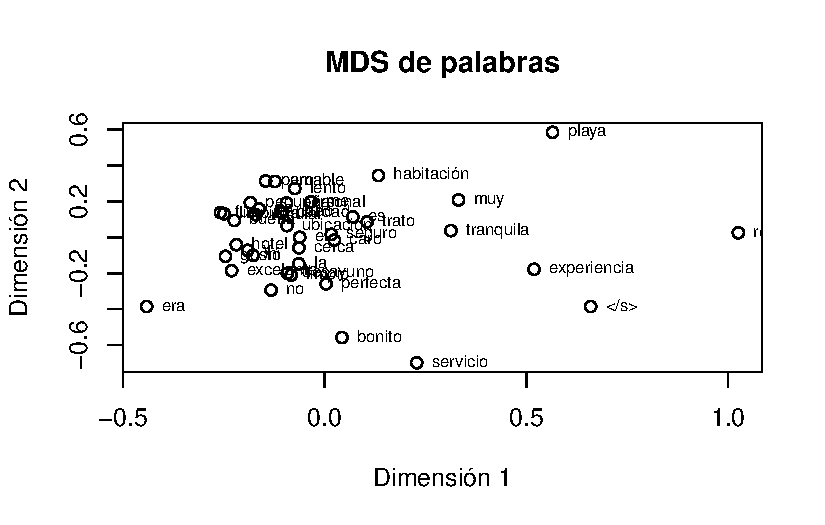
\includegraphics[keepaspectratio]{carga_datos_files/figure-pdf/unnamed-chunk-26-1.pdf}}

\bookmarksetup{startatroot}

\chapter{Anáilsis Aplec Tom 1 1915segunda
edición}\label{anuxe1ilsis-aplec-tom-1-1915segunda-ediciuxf3n}

Analizamos en este capítulo el tomo I de 1915, edición dos, que se
encuentra en la carpeta \texttt{raw\_text} los ficheros de interes son.

\begin{Shaded}
\begin{Highlighting}[]
\FunctionTok{list.files}\NormalTok{(}\StringTok{"raw\_text/"}\NormalTok{, }\AttributeTok{pattern =} \StringTok{"tomo1"}\NormalTok{, }\AttributeTok{ignore.case =} \ConstantTok{TRUE}\NormalTok{, }\AttributeTok{full.names =} \ConstantTok{TRUE}\NormalTok{)}
\end{Highlighting}
\end{Shaded}

\begin{verbatim}
[1] "raw_text/rondalles_ocr_tomo1.csv" "raw_text/rondalles_ocr_tomo1.rds"
[3] "raw_text/rondalles_ocr_tomo1.txt" "raw_text/tabla_tomo1.csv"        
\end{verbatim}

El fichero .csv contiene un data frame con las páginas del Tomo 1. Este
fichero incluye el número de página real: la página 1 corresponde a la
portada y la numeración continúa de forma consecutiva hasta el final,
con un total de 300 páginas. Esta numeración no coincide con la de la
edición, que utiliza numeración romana para el preámbulo y numeración
arábiga para las rondallas. Por otro lado, el fichero .txt contiene el
texto en formato raw codificado en UTF-8, con un separador de páginas
del tipo:

\begin{verbatim}
=== Página 1 ===
presented by
Mrs B. Huelin, l
on bebalfof the late
Mr D.S. Huelin
Mar- 2002
CARA Lo


=== Página 2 ===
RONDATES MALLORQUINES


=== Página 3 ===
APLEC
DE
È D'EN
JORDI DES RECÓ
(ANTONI M2 ALCOVER: PRE.)
SEGONA EDICIÓ
TOM I
AMB LLECENCIA DE L' ORDINARI
CIUTAT DE MALLORCA
ESTAMPA D' Es SBBASTIA P1ZA
(915

\end{verbatim}

Leemos estos dos ficheros

\begin{Shaded}
\begin{Highlighting}[]
\NormalTok{tomo1 }\OtherTok{\textless{}{-}} \FunctionTok{read\_csv}\NormalTok{(}\StringTok{"raw\_text/rondalles\_ocr\_tomo1.csv"}\NormalTok{)}
\end{Highlighting}
\end{Shaded}

\begin{verbatim}
Rows: 300 Columns: 3
-- Column specification --------------------------------------------------------
Delimiter: ","
chr (1): texto
dbl (1): pagina
lgl (1): error

i Use `spec()` to retrieve the full column specification for this data.
i Specify the column types or set `show_col_types = FALSE` to quiet this message.
\end{verbatim}

\begin{Shaded}
\begin{Highlighting}[]
\NormalTok{tabla}\OtherTok{\textless{}{-}} \FunctionTok{read\_csv}\NormalTok{(}\StringTok{"raw\_text/tabla\_tomo1.csv"}\NormalTok{)}
\end{Highlighting}
\end{Shaded}

\begin{verbatim}
Rows: 27 Columns: 4
-- Column specification --------------------------------------------------------
Delimiter: ","
chr (2): linea, titulo
dbl (2): pagina, indice

i Use `spec()` to retrieve the full column specification for this data.
i Specify the column types or set `show_col_types = FALSE` to quiet this message.
\end{verbatim}

Veamos el contenido de ambos data frames

\begin{Shaded}
\begin{Highlighting}[]
\FunctionTok{glimpse}\NormalTok{(tomo1)}
\end{Highlighting}
\end{Shaded}

\begin{verbatim}
Rows: 300
Columns: 3
$ pagina <dbl> 1, 2, 3, 4, 5, 6, 7, 8, 9, 10, 11, 12, 13, 14, 15, 16, 17, 18, ~
$ texto  <chr> "presented by\r\nMrs B. Huelin, l\r\non bebalfof the late\r\nMr~
$ error  <lgl> NA, NA, NA, NA, NA, NA, NA, NA, NA, NA, NA, NA, NA, NA, NA, NA,~
\end{verbatim}

\begin{Shaded}
\begin{Highlighting}[]
\FunctionTok{all}\NormalTok{(}\FunctionTok{is.na}\NormalTok{(tomo1}\SpecialCharTok{$}\NormalTok{error))}
\end{Highlighting}
\end{Shaded}

\begin{verbatim}
[1] TRUE
\end{verbatim}

Contiene tres columnas: ``pagina'', ``texto'' y ``error''. La columna
``pagina'' indica el número de página, la columna ``texto'' contiene el
texto extraído mediante OCR, y la columna ``error'' indica si hubo algún
error durante el proceso de OCR para esa página, todos están a
\texttt{NA}no ha habido errores.

Ahota leemos el índice

\begin{Shaded}
\begin{Highlighting}[]
\NormalTok{knitr}\SpecialCharTok{::}\FunctionTok{kable}\NormalTok{(tabla)}
\end{Highlighting}
\end{Shaded}

{\def\LTcaptype{none} % do not increment counter
\begin{longtable}[]{@{}
  >{\raggedright\arraybackslash}p{(\linewidth - 6\tabcolsep) * \real{0.4800}}
  >{\raggedleft\arraybackslash}p{(\linewidth - 6\tabcolsep) * \real{0.0700}}
  >{\raggedright\arraybackslash}p{(\linewidth - 6\tabcolsep) * \real{0.3800}}
  >{\raggedleft\arraybackslash}p{(\linewidth - 6\tabcolsep) * \real{0.0700}}@{}}
\toprule\noalign{}
\begin{minipage}[b]{\linewidth}\raggedright
linea
\end{minipage} & \begin{minipage}[b]{\linewidth}\raggedleft
pagina
\end{minipage} & \begin{minipage}[b]{\linewidth}\raggedright
titulo
\end{minipage} & \begin{minipage}[b]{\linewidth}\raggedleft
indice
\end{minipage} \\
\midrule\noalign{}
\endhead
\bottomrule\noalign{}
\endlastfoot
Portada e INICIO & 1 & Portada e INICIO & 1 \\
PROLEG DE LA 1. & 5 & PROLEG DE LA 1. & 5 \\
PROLEG DE LA 2. & 16 & PROLEG DE LA 2. & 16 \\
EN JUANET I ES SET MISSATGES 1 & 1 & EN JUANET I ES SET MISSATGES &
26 \\
UN FESTETJADOR. 19 & 19 & UN FESTETJADOR. & 44 \\
S' HERMOSURA DEL MON 23 & 23 & S' HERMOSURA DEL MON & 48 \\
SA FIA DES CARBONERET 35 & 35 & SA FIA DES CARBONERET & 60 \\
EN MARTÍ TACÓ . 44 & 44 & EN MARTÍ TACÓ . & 69 \\
ES CA D'EN BUA I ES MOIX D'EN PEJULÍ. 57 & 57 & ES CA D'EN BUA I ES MOIX
D'EN PEJULÍ. & 82 \\
N'ESTEL D' OR 63 & 63 & N'ESTEL D' OR & 88 \\
NA MAGRANETA. 84 & 84 & NA MAGRANETA. & 109 \\
SA JAIA XELOC I SA JAIA BIGALOT 99 & 99 & SA JAIA XELOC I SA JAIA
BIGALOT & 124 \\
EN JUANET DE SA GERRA 107 & 107 & EN JUANET DE SA GERRA & 132 \\
ES TRES GERMANS I ES NOU GEGANTS. 114 & 114 & ES TRES GERMANS I ES NOU
GEGANTS. & 139 \\
EN PERE DE SA BUTZA 128 & 128 & EN PERE DE SA BUTZA & 153 \\
ES SET CEROS 133 & 133 & ES SET CEROS & 158 \\
ES SEGADOR I SA BEATA 146 & 146 & ES SEGADOR I SA BEATA & 171 \\
EN SALOM I ES BAL'LE. 150 & 150 & EN SALOM I ES BAL'LE. & 175 \\
N AGRACIAT 165 & 165 & N AGRACIAT & 190 \\
ES CASTELL D'IRÁS I NO TORNARÁS 174 & 174 & ES CASTELL D'IRÁS I NO
TORNARÁS & 199 \\
Es QUATRE GERMANS 213 & 213 & Es QUATRE GERMANS & 238 \\
S' HOMO I ES LLEÓ 228 & 228 & S' HOMO I ES LLEÓ & 253 \\
N' ESPARDENYETА 231 & 231 & N' ESPARDENYETА & 256 \\
Es DOs BESSONS 244 & 244 & Es DOs BESSONS & 269 \\
SA RABOA I S' ERISSÓ 256 & 256 & SA RABOA I S' ERISSÓ & 281 \\
SA RONDAIA D' EN VIT 269 & 269 & SA RONDAIA D' EN VIT & 294 \\
BON-JESÚS I ETS ALTRES APÒSTOLS.. 273 & 273 & BON-JESÚS I ETS ALTRES
APÒSTOLS.. & 298 \\
\end{longtable}
}

Las variables son ``linea'', ``pagina'', ``titulo'' e ``indice''. La
variable ``linea'' contiene el título de cada sección o capítulo, la
variable ``pagina'' indica la página en la que se encuentra esa sección
o capítulo, la variable ``titulo'' es una copia de ``linea'' y la
variable ``indice'' indica el número de página real en el documento, que
NO se corresponde con la numeración del tomo.

\bookmarksetup{startatroot}

\chapter{Corpus Tomo 1}\label{corpus-tomo-1}

Construyamos el corpus de este aplec separando cada capítulo

\begin{Shaded}
\begin{Highlighting}[]
\NormalTok{corpus\_tomo1 }\OtherTok{\textless{}{-}}\NormalTok{ tabla }\SpecialCharTok{\%\textgreater{}\%}
  \FunctionTok{mutate}\NormalTok{(}
    \AttributeTok{texto =} \FunctionTok{map2\_chr}\NormalTok{(}
\NormalTok{      indice,}
      \FunctionTok{lead}\NormalTok{(indice, }\AttributeTok{default =} \FunctionTok{nrow}\NormalTok{(tomo1) }\SpecialCharTok{+} \DecValTok{1}\NormalTok{),}
      \SpecialCharTok{\textasciitilde{}}\NormalTok{ \{}
\NormalTok{        start }\OtherTok{\textless{}{-}}\NormalTok{ .x}
\NormalTok{        end }\OtherTok{\textless{}{-}}\NormalTok{ .y }\SpecialCharTok{{-}} \DecValTok{1}
\NormalTok{        page\_texts }\OtherTok{\textless{}{-}}\NormalTok{ tomo1 }\SpecialCharTok{\%\textgreater{}\%}
          \FunctionTok{filter}\NormalTok{(pagina }\SpecialCharTok{\textgreater{}=}\NormalTok{ start, pagina }\SpecialCharTok{\textless{}}\NormalTok{ end) }\SpecialCharTok{\%\textgreater{}\%}
          \FunctionTok{pull}\NormalTok{(texto)}
        \FunctionTok{paste}\NormalTok{(page\_texts, }\AttributeTok{collapse =} \StringTok{"}\SpecialCharTok{\textbackslash{}n}\StringTok{"}\NormalTok{)}
\NormalTok{      \}}
\NormalTok{    )}
\NormalTok{  ) }\SpecialCharTok{\%\textgreater{}\%}
  \FunctionTok{select}\NormalTok{(linea, pagina, titulo, texto)}
\end{Highlighting}
\end{Shaded}

La rondalla más corta es la número 4 que está en la entrada 7 de la
tibble , que se titula ``Rondalla de la filla del rei de les flors''.
Veamos su texto

\begin{Shaded}
\begin{Highlighting}[]
\FunctionTok{cat}\NormalTok{(}\FunctionTok{head}\NormalTok{(corpus\_tomo1}\SpecialCharTok{$}\NormalTok{texto[}\DecValTok{7}\NormalTok{]))}
\end{Highlighting}
\end{Shaded}

\begin{verbatim}
P ecaomos ame dopoec entens mb
SA FIA DES CARBONERET '
——bo— De ea ——

a IXÒ era un carboner que tenía un fil, una

GA fia casada i dues tadrines.
LS Un dia el Rei, cassant cassant, passa
per davant sa barraca des carboner, i troba sa seua
fia darrera, una fadrineta de setze anys, sa més
galanxona, que havía nom Catalineta.

El Rei, com la va veure, va romandre embadalit,
ili digué:

—Alabat sía Deu. l

—Pera sempre, senyor Reit diu s' al'lotona.

—e Quina la tas2 diu el Rei.

— Quin damunt davall són, diu ella.

—j Damunt davall són/ s'esclamà el Rei, i repa-
rà una Sarria que feia embalum.

—eQue hi ha dins aquella sarria2 demanà.

—Xerrim baix, digué Na Catalineta.

—j Xerrim baixl 's' esclamà el Rei, sense que li
ocorregués que poría esser allò i va dir: — -

—éA on ès ton pare

— A treure gent de ca-seua, diu ella.

Il La'm contú la mateixa criada de ca-nostra, N' Antonina Cordera.

36 RONDAIES MALLORQUINES
o —èl ta mare2 diu el Rei. :

—À plorar es pler de l any passat, respòn s' al-
lota.

—el es teu germà2 diu el Rei.

—A cassar. Deixa sa cassa que ha agafada,
i du sa que no ha poguda agafar, diu ella.

El Rei quedà tot contús amb aquesta partida d2
coses que aquella pitxorina li havía entlocades.

—bDiràs a ton pare que venga es vespre a veu-
re 'm, li digué i se 'n anà.

Es vespre es carboner se presenta a ca 1 Rei, i
diu:
ee —BEona nittenga, senyor Rei. cEstà bonet2 Que
vol de mí2 :
ee —Bo estic, gracies a Deu, diu el Rei. Som pas-
sat avui per sa teua barraca, i tens una tia més
viva que una centella: Li he tetes un parei de pre-
guntes, i m' ha respost d'una manera que m' ha
deixat 'contús: M'ha dit que cuinavà damunt davall
són.

—Tenía "raó, diu es carboner: Eren ciurons,
que, quant $' olla bull, pugen i davallen, i un cop
són damunt i un cop davall.

—iEl diantre ès aquesta al'lotal diu el Rei. I m'
ha dit també que dins una sarria hi havía .xerrim
baix.

—Es verl diu es carboner: e-hi havía s' altra fia
despuiada, perque totes dues no més tenen un
vestit, el duen un dia per.hom, i Sa qui no 'l du, es-
tà dins sa sarria, i, en venir ningú estern, xerra
baix, porque no se temin d'ella.

—i El diantre es aquesta al'lotal diu el Rei. Í m'
ha dit llavò que tu eres a treure gent de ca-seua.
' —Es ver, diu es carboner: era a treure rabas-
sons.

SA FIA DES CARBONERET 37
—iSí que endevinava idòl diu el Rei. I llavò m'
ha dit que sa mare era a plorar es pler de l any
passat. Ú
—I massa que hi eral diu es carboner. Entany .
casérem una tia, i despuisahir se morí, al cel sía
ella i tots los morts, i sa dona hi era, ja hu veu,
per donar cap. Í ella i noltros ploràvem. i . ploram,
es pler que l'any passat tenguérem des casament. L
l es carbòneret va rompre en plors. —, ..— ,,
—No plores, digué el Rei. Deu ho ha fet, i ell
sab que fa, i no pot errar. Una altra cosa'm' ha
dita aquella polisseta, i ès sa que m' ha deixat més
contús. M' ha dit que es seu germà. era a, cassar,.
i que deixava sa cassa que havía agafada, i duia
sa que no havía poguda agafar... ,A veure qui hu
entén an aixòl dèy
—Jo le hi diré, diu es carboner: era a esplugar-
se: deixava morts es pois qne agafava, i duia da-
munt el còs tots es qui no havía poguts agatar.
—i El diantre es aquesta al'lotal digué el Rei tot
admirat. Mira, si no la puc contondre, m'he :de
casar. amb ella. 1 P a
l eque ta ell Àgata tres ous, los trenca dins, un
plat, los rebat una bona estona i diu an .es carbo-
neret. l id
—Jèsi du aquests ous a sa teua tia. Que, les pos,
i tendrem aviram en casar-mos. o Res ay
—iPobre tieta meual scom n'ha de sortir: .d'
aquesta2 deia es carboneret quant. se "n ternaya a
sa barraca. : d'AS qe
E-hi arriba, conta es pas a sa ,fia, i ella .s'ex-
clama: pat
—PD' això estau embarassat2. Esperau, veureu.
Agata unes quantes grapades de civada, la mol
ben mòlta, i li diu:

38 RONDAIES MALLORQUINES

e—Jau aquesta farina. Duis-la an el Rei. Que la
sembr, i tendrem civada per dar a s'aviram en
casar-mos.

- Es carboneret se'n hi va, va fer sa comanda de
Na Catalina, i el Rei va quedar sense paraula.

4 Després de pensar-hi molt, pren un tros de. roba,
el fa bocins menuts menuts, com una ungla.

—Jès, li digué. Du-los a sa teua fia, que tassa
es menudai per quant mos casem i tenguem cap
infant. :

: —3jPobre tieta meual ccom n'ha de sortir d'
aquestal deia es carboneret tot enfadat, quant se
en:tornava a sa barraca. ds
 E-hi arriba, dona a Na Catalineta sa comanda
del Rei, i ella s' exclama:

—dAixò ès tot

Agafa un parei d' ensenais, los esmenuca tot lo
que pot, los dona a son pare, i li diu:

—Jau, duis-los an el Rei, i que 'n tassa 's bres
per un Si a cas...

Ell ja ès partit cap a ca I Rei, li dona sa coman-
da de Na Catalina, i el Rei iquè havía de sebre
respondrel Se: posa pensa qui pensa, per veure
com l'apuraría, i a la fi, pren un paner, i diu: l

—Jès, du 'l a sa teua fia, i que l'umpli de riaies.

—iPobre fia meual jaquesta vegada no 'n surtl
deia es carboneret, tornant-se 'n a. sa barraca. l
amb so cap dins es paner se posava after ija ja jal
riu que riu amb unes riaies lo més forsades, i jque
havía d'omplires panerl i Tant com es moix

Tot-d' una que arriba í Na Catalineta el sent,
li diu:

—iD' això estau embarassatP Anau a agatar tres
dotzenes d' aucellons. Los posau . dins aquest pa-

SA FIA DES CARBONERET 39
ner, tapau damunt amb un pedàs, vos n'anau a
ca 'l Rei, esperau que estiga en taula, li entregau
es paner de part meua, i que 'l destap.

Es carboneret e-hu va fer així. Justament el Rei
tenía una bona partida de convidats. Fa destapar
es paner, surt aquell esbart d' aucellons, i uns. se
tiren per dalt ses gerretes de s'aigo i es garrafs
de ví, altres voletetjant feren plats i tassons, altres
peguen per demunt es cap i ses espal'les des con-
vidats, altres los freguen amb ses ales, front, gal-
tes i oreies, i hi hagué qualque nas afavorit. que

se'n va dur més d'un quern de: titorades, i ven-
guen esquitxos, i raigs, i rois, taques, i crits, i
renou, i tot-hom no pogué estar que no esclafís
de riure, i cuidaden a ter ui de riaies.:

/ El Rei, apurat de tot, veent que sempre queda-
va davall, a torsa de sucar ets ais, se 'n va treure
una que se creia que havía de capturar sa carbo-
nereta..—

—No res, va dir a son pare. Diga-li que venga
ni vestida ni sensa vestir, ni pes camí ni fora
camí, ni cualcant ni a peu.

—jPobre tia meual jAquesta vegada no 'n surtsi
deia es carboneret, tot entadat, tornant-se 'n a sa
barraca.

Quant e-hi va esser, i Na Catalina el sentí, li
diu:

—eD' això estau embarassat2 Anau a Ses Pla-
nes, menau un boc muntanyenc, ben seuvatgí.

Son pare hi va, compra es boc, i le hi mena.
Ella se desmuda, s'embolica un filacs, se posa
damunt s' animal, i ja es partida cap a ca 'l Rei.

1 Possessió de Sant Llorens des Cardessar.

3

4) Ò RONDAIES MALLORQUINES
I Es boc, ja hu. crec, feia bots.i escaravits, i tot eren
fues i xecalines. Assetsuaixí servava camí, asset-
suaixí no 'n servava: la tomava, ella s' hi tornava:
posar damunt: i la tornava tomar, i ella s' hi tor-
nava posar.

De manera que ni anava vestida ni sensa vestir,

ni p'es camí ni tora camí, ni cualcant ni a peu.
—El-Rei, com la va veure, digué:

—Paraula de Rei no pot mentir. No t' he poguda
confondre: mos hem de casar.

—BEll que hu véssem, va dir ella.

—Aviat ho veurem, si Deu ho vol, diu el Rei. È
Però va amb uns pactes.

—eQuins pactes son aquests2 diu ella.

—Que no pots donar conseis a negú, diu el Rei.
Si 'n dones cap, te 'n hauràs de tornar a sa barraca
de ton pare.

—gl no me 'n he de porer dur resè diu ella.

—Vaja, per que no 't pugues queixar, te'n po-
dràs dur una joia, diu el Rei.

—iUna no mésP égrossa o petitaP diu ella.

—No res, sa que tu voldràs, diu el Rei.

Ella hiipensé'una estoneta, i s' exclama: .,

— Feta està sa barrina. /

Se casaren, el Rei tirà sa casa per sa finestra,
e-hi hagué un:ast i olla de lo més alt de punt, i
es sarau que 'S va fer no hu poren dir persones
nades.

Des cap d'una mesada, amàú a ròmandre a ca ll
Rei un mahonès amb una ego.

—eA on pos aquesta: bistietaP digué. ,

—Dins s' estable, li varen respondre.

: E-hi guaita, i hi veu un cavall, i diu:

—eQue l'he de posar devora es cavall2

SA FIA DES CARBONERET 41

—Posau-le-hi, li varen dir...

Lla hi posà. ,

Lo endemóà matí s' ego va haver feta una pollina::
o 3 El Rei la volía, perque. deia que, essent nada
dins s' estable a on no hi havía altra bistia seua
més que es cavall, per forsa l'havía d' haver feta

es cavall.

—Pero isi hi havía s' ego des mahonèsi li deien.

—No m'empatx de raons, deia ell. No m'heu
de dir voltros a on ès el Carme ni el Sant Esperit.
Jo no tenía altra bistia dins s'estable, cès nada
una pollina2 Idò ès des cavall. É

Es criats, com el veren tan encabotat, el deixa-
ren anar. R

Es mahonès anà també ben alerta a fer-li
cuantra.

La Reina hu va sebre, i li mostra una bassa seca
que hi havía allà aprop, i li diu:

l —Anau-hi amb una canyeta i una ginya, i teis

com que pescar. El Rei, en anar-se'n a sa cassada,

en .passarà, i vos dirà:—eQue feis2 Il heu de dir:

—Pesc. —cQue pescau2 dirà ell. —Sardines, heu

de dir vos. —eQuin possible ès, dirà ell, sensa aigo

a sa bassa, pescar-hi sardines2 I vos: heu de dir:

—Tant possible ès, sensa haver-hi aigo, agafar-hi
sardines, com que un cavall fassa pollines.

Es mahonès seguí es consei de la Reina.

Passà el Rei per devora sa bassa, el veu amb sa
canyeta i sa ginya lo mateix d'un pescador que
espera una gran peixetada, i li diu: pea

—el. ara que tas

—Pescl diu es mahonès. us

—eiQuè pesquesP diu el Rei, ,

—Sardinesi diu es mahonès. qe ES de

42 RONDAIES MALLORQUINES

—jDe tros de banci diu el. Rei. iNo hi ha una
gota..d'aigo dins sa bassa, i hi vols agafar sardi-
nesl équin possible es que n' agatis cap2

—Tant possible ès, digué es mahonès, sensa
haver-hi aigo agatar-hi sardines, com que un cavall
fassa pollines.

El Rei va quedar taiat davant aquesta sortida, i
per desfer-se d'aquells trumíos, digué:

—Anau a ca-meua, i menau-vos-ne s' ego i sa
pollina i espitxau-vos més que de pressa cap a.ca-
vostra.

Es mahonès e-hu va ter així, i el Rei pensà en-
tre sí mateix:

—Ja ès la Reina que li ha aconseiat que "m fés
aquesta.

Gira en redó cap a ca-seua, i li diu:

—Ets tu. Negú pot esser més que tu.

—gl ara2 diu la Reina. I /

—Suaral diu el Rei. Has donat un consei an es
mahonès: no hu pots negar..

—Le hi he donat per que no. tesses s' injusticia.
de prendre-li sa pollinal diu la Reina.

—No m' empatx de raonsi diu el Rei. L' has do-
nat i no 'l poríes donar. éSabs quins son es pactes
que 't vaig posar quant mos casàrem2

—Síl. diu la Reina.

—lIdò te 'n pots anar en volert diu el Rei...

—ç Que no porem dinar abans2 diu la Reina.

—No res idò, diu el Rei: dinarem, i llavò te 'n
aniràs.

Dinaren, i sa traidora li donà dormissons.

Quant el tengué ben adormit, ta enganxar es
cotxo, le hi posa de dins, i dona orde de partir cap
a sa'barraca de son pare.
\end{verbatim}

Cómo se ve el tla OCR ha funcionado bastante bien, aunque hay algunos
errores de reconocimiento, como ``RONDATES'' en lugar de ``RONDALLES'' o
``MAYORQUINES'' en lugar de ``MALLORQUINES''. Sin embargo, el texto es
legible y se puede trabajar con él para realizar análisis posteriores.

Podéis curar lo errores más fáciles con ecpresiones regulares

Por ejemplo, para corregir ``RONDATES'' a ``RONDALLES'' y
``MAYORQUINES'' a ``MALLORQUINES'', podríamos usar el siguiente código:

\begin{Shaded}
\begin{Highlighting}[]
\NormalTok{corpus\_tomo1 }\OtherTok{\textless{}{-}}\NormalTok{ corpus\_tomo1 }\SpecialCharTok{\%\textgreater{}\%}
  \FunctionTok{mutate}\NormalTok{(}
    \AttributeTok{texto =} \FunctionTok{str\_replace\_all}\NormalTok{(texto, }\FunctionTok{c}\NormalTok{(}
      \StringTok{"RONDATES"} \OtherTok{=} \StringTok{"RONDALLES"}\NormalTok{,}
      \StringTok{"MAYORQUINES"} \OtherTok{=} \StringTok{"MALLORQUINES"}
\NormalTok{    ))}
\NormalTok{  )}
\end{Highlighting}
\end{Shaded}

\begin{verbatim}
—No m' empatx de raonsi diu el Rei. L' has do-
nat i no 'l poríes donar. éSabs quins son es pactes
que 't vaig posar quant mos casàrem2
\end{verbatim}

Por ejemplo aquí podríamos corregir los silabeados como ``don-at'' en el
fin de linea con el siguiente código para corta palabra partidas de esta
manera:

\begin{Shaded}
\begin{Highlighting}[]
\FunctionTok{library}\NormalTok{(stringr)}
\NormalTok{corpus\_tomo1 }\OtherTok{\textless{}{-}}\NormalTok{ corpus\_tomo1 }\SpecialCharTok{\%\textgreater{}\%}
  \FunctionTok{mutate}\NormalTok{(}
    \AttributeTok{texto =} \FunctionTok{str\_replace\_all}\NormalTok{(texto, }\StringTok{"(}\SpecialCharTok{\textbackslash{}\textbackslash{}}\StringTok{p\{L\}+){-}}\SpecialCharTok{\textbackslash{}\textbackslash{}}\StringTok{s*}\SpecialCharTok{\textbackslash{}\textbackslash{}}\StringTok{n}\SpecialCharTok{\textbackslash{}\textbackslash{}}\StringTok{s*(}\SpecialCharTok{\textbackslash{}\textbackslash{}}\StringTok{p\{L\}+)"}\NormalTok{, }\StringTok{"}\SpecialCharTok{\textbackslash{}\textbackslash{}}\StringTok{1}\SpecialCharTok{\textbackslash{}\textbackslash{}}\StringTok{2"}\NormalTok{)}
\NormalTok{  )}
\end{Highlighting}
\end{Shaded}

Efectivamente ahora

\begin{Shaded}
\begin{Highlighting}[]
\FunctionTok{cat}\NormalTok{(}\FunctionTok{head}\NormalTok{(corpus\_tomo1}\SpecialCharTok{$}\NormalTok{texto[}\DecValTok{7}\NormalTok{]))}
\end{Highlighting}
\end{Shaded}

\begin{verbatim}
P ecaomos ame dopoec entens mb
SA FIA DES CARBONERET '
——bo— De ea ——

a IXÒ era un carboner que tenía un fil, una

GA fia casada i dues tadrines.
LS Un dia el Rei, cassant cassant, passa
per davant sa barraca des carboner, i troba sa seua
fia darrera, una fadrineta de setze anys, sa més
galanxona, que havía nom Catalineta.

El Rei, com la va veure, va romandre embadalit,
ili digué:

—Alabat sía Deu. l

—Pera sempre, senyor Reit diu s' al'lotona.

—e Quina la tas2 diu el Rei.

— Quin damunt davall són, diu ella.

—j Damunt davall són/ s'esclamà el Rei, i reparà una Sarria que feia embalum.

—eQue hi ha dins aquella sarria2 demanà.

—Xerrim baix, digué Na Catalineta.

—j Xerrim baixl 's' esclamà el Rei, sense que li
ocorregués que poría esser allò i va dir: — -

—éA on ès ton pare

— A treure gent de ca-seua, diu ella.

Il La'm contú la mateixa criada de ca-nostra, N' Antonina Cordera.

36 RONDAIES MALLORQUINES
o —èl ta mare2 diu el Rei. :

—À plorar es pler de l any passat, respòn s' allota.

—el es teu germà2 diu el Rei.

—A cassar. Deixa sa cassa que ha agafada,
i du sa que no ha poguda agafar, diu ella.

El Rei quedà tot contús amb aquesta partida d2
coses que aquella pitxorina li havía entlocades.

—bDiràs a ton pare que venga es vespre a veure 'm, li digué i se 'n anà.

Es vespre es carboner se presenta a ca 1 Rei, i
diu:
ee —BEona nittenga, senyor Rei. cEstà bonet2 Que
vol de mí2 :
ee —Bo estic, gracies a Deu, diu el Rei. Som passat avui per sa teua barraca, i tens una tia més
viva que una centella: Li he tetes un parei de preguntes, i m' ha respost d'una manera que m' ha
deixat 'contús: M'ha dit que cuinavà damunt davall
són.

—Tenía "raó, diu es carboner: Eren ciurons,
que, quant $' olla bull, pugen i davallen, i un cop
són damunt i un cop davall.

—iEl diantre ès aquesta al'lotal diu el Rei. I m'
ha dit també que dins una sarria hi havía .xerrim
baix.

—Es verl diu es carboner: e-hi havía s' altra fia
despuiada, perque totes dues no més tenen un
vestit, el duen un dia per.hom, i Sa qui no 'l du, està dins sa sarria, i, en venir ningú estern, xerra
baix, porque no se temin d'ella.

—i El diantre es aquesta al'lotal diu el Rei. Í m'
ha dit llavò que tu eres a treure gent de ca-seua.
' —Es ver, diu es carboner: era a treure rabassons.

SA FIA DES CARBONERET 37
—iSí que endevinava idòl diu el Rei. I llavò m'
ha dit que sa mare era a plorar es pler de l any
passat. Ú
—I massa que hi eral diu es carboner. Entany .
casérem una tia, i despuisahir se morí, al cel sía
ella i tots los morts, i sa dona hi era, ja hu veu,
per donar cap. Í ella i noltros ploràvem. i . ploram,
es pler que l'any passat tenguérem des casament. L
l es carbòneret va rompre en plors. —, ..— ,,
—No plores, digué el Rei. Deu ho ha fet, i ell
sab que fa, i no pot errar. Una altra cosa'm' ha
dita aquella polisseta, i ès sa que m' ha deixat més
contús. M' ha dit que es seu germà. era a, cassar,.
i que deixava sa cassa que havía agafada, i duia
sa que no havía poguda agafar... ,A veure qui hu
entén an aixòl dèy
—Jo le hi diré, diu es carboner: era a esplugarse: deixava morts es pois qne agafava, i duia damunt el còs tots es qui no havía poguts agatar.
—i El diantre es aquesta al'lotal digué el Rei tot
admirat. Mira, si no la puc contondre, m'he :de
casar. amb ella. 1 P a
l eque ta ell Àgata tres ous, los trenca dins, un
plat, los rebat una bona estona i diu an .es carboneret. l id
—Jèsi du aquests ous a sa teua tia. Que, les pos,
i tendrem aviram en casar-mos. o Res ay
—iPobre tieta meual scom n'ha de sortir: .d'
aquesta2 deia es carboneret quant. se "n ternaya a
sa barraca. : d'AS qe
E-hi arriba, conta es pas a sa ,fia, i ella .s'exclama: pat
—PD' això estau embarassat2. Esperau, veureu.
Agata unes quantes grapades de civada, la mol
ben mòlta, i li diu:

38 RONDAIES MALLORQUINES

e—Jau aquesta farina. Duis-la an el Rei. Que la
sembr, i tendrem civada per dar a s'aviram en
casar-mos.

- Es carboneret se'n hi va, va fer sa comanda de
Na Catalina, i el Rei va quedar sense paraula.

4 Després de pensar-hi molt, pren un tros de. roba,
el fa bocins menuts menuts, com una ungla.

—Jès, li digué. Du-los a sa teua fia, que tassa
es menudai per quant mos casem i tenguem cap
infant. :

: —3jPobre tieta meual ccom n'ha de sortir d'
aquestal deia es carboneret tot enfadat, quant se
en:tornava a sa barraca. ds
 E-hi arriba, dona a Na Catalineta sa comanda
del Rei, i ella s' exclama:

—dAixò ès tot

Agafa un parei d' ensenais, los esmenuca tot lo
que pot, los dona a son pare, i li diu:

—Jau, duis-los an el Rei, i que 'n tassa 's bres
per un Si a cas...

Ell ja ès partit cap a ca I Rei, li dona sa comanda de Na Catalina, i el Rei iquè havía de sebre
respondrel Se: posa pensa qui pensa, per veure
com l'apuraría, i a la fi, pren un paner, i diu: l

—Jès, du 'l a sa teua fia, i que l'umpli de riaies.

—iPobre fia meual jaquesta vegada no 'n surtl
deia es carboneret, tornant-se 'n a. sa barraca. l
amb so cap dins es paner se posava after ija ja jal
riu que riu amb unes riaies lo més forsades, i jque
havía d'omplires panerl i Tant com es moix

Tot-d' una que arriba í Na Catalineta el sent,
li diu:

—iD' això estau embarassatP Anau a agatar tres
dotzenes d' aucellons. Los posau . dins aquest paSA FIA DES CARBONERET 39
ner, tapau damunt amb un pedàs, vos n'anau a
ca 'l Rei, esperau que estiga en taula, li entregau
es paner de part meua, i que 'l destap.

Es carboneret e-hu va fer així. Justament el Rei
tenía una bona partida de convidats. Fa destapar
es paner, surt aquell esbart d' aucellons, i uns. se
tiren per dalt ses gerretes de s'aigo i es garrafs
de ví, altres voletetjant feren plats i tassons, altres
peguen per demunt es cap i ses espal'les des convidats, altres los freguen amb ses ales, front, galtes i oreies, i hi hagué qualque nas afavorit. que

se'n va dur més d'un quern de: titorades, i venguen esquitxos, i raigs, i rois, taques, i crits, i
renou, i tot-hom no pogué estar que no esclafís
de riure, i cuidaden a ter ui de riaies.:

/ El Rei, apurat de tot, veent que sempre quedava davall, a torsa de sucar ets ais, se 'n va treure
una que se creia que havía de capturar sa carbonereta..—

—No res, va dir a son pare. Diga-li que venga
ni vestida ni sensa vestir, ni pes camí ni fora
camí, ni cualcant ni a peu.

—jPobre tia meual jAquesta vegada no 'n surtsi
deia es carboneret, tot entadat, tornant-se 'n a sa
barraca.

Quant e-hi va esser, i Na Catalina el sentí, li
diu:

—eD' això estau embarassat2 Anau a Ses Planes, menau un boc muntanyenc, ben seuvatgí.

Son pare hi va, compra es boc, i le hi mena.
Ella se desmuda, s'embolica un filacs, se posa
damunt s' animal, i ja es partida cap a ca 'l Rei.

1 Possessió de Sant Llorens des Cardessar.

3

4) Ò RONDAIES MALLORQUINES
I Es boc, ja hu. crec, feia bots.i escaravits, i tot eren
fues i xecalines. Assetsuaixí servava camí, assetsuaixí no 'n servava: la tomava, ella s' hi tornava:
posar damunt: i la tornava tomar, i ella s' hi tornava posar.

De manera que ni anava vestida ni sensa vestir,

ni p'es camí ni tora camí, ni cualcant ni a peu.
—El-Rei, com la va veure, digué:

—Paraula de Rei no pot mentir. No t' he poguda
confondre: mos hem de casar.

—BEll que hu véssem, va dir ella.

—Aviat ho veurem, si Deu ho vol, diu el Rei. È
Però va amb uns pactes.

—eQuins pactes son aquests2 diu ella.

—Que no pots donar conseis a negú, diu el Rei.
Si 'n dones cap, te 'n hauràs de tornar a sa barraca
de ton pare.

—gl no me 'n he de porer dur resè diu ella.

—Vaja, per que no 't pugues queixar, te'n podràs dur una joia, diu el Rei.

—iUna no mésP égrossa o petitaP diu ella.

—No res, sa que tu voldràs, diu el Rei.

Ella hiipensé'una estoneta, i s' exclama: .,

— Feta està sa barrina. /

Se casaren, el Rei tirà sa casa per sa finestra,
e-hi hagué un:ast i olla de lo més alt de punt, i
es sarau que 'S va fer no hu poren dir persones
nades.

Des cap d'una mesada, amàú a ròmandre a ca ll
Rei un mahonès amb una ego.

—eA on pos aquesta: bistietaP digué. ,

—Dins s' estable, li varen respondre.

: E-hi guaita, i hi veu un cavall, i diu:

—eQue l'he de posar devora es cavall2

SA FIA DES CARBONERET 41

—Posau-le-hi, li varen dir...

Lla hi posà. ,

Lo endemóà matí s' ego va haver feta una pollina::
o 3 El Rei la volía, perque. deia que, essent nada
dins s' estable a on no hi havía altra bistia seua
més que es cavall, per forsa l'havía d' haver feta

es cavall.

—Pero isi hi havía s' ego des mahonèsi li deien.

—No m'empatx de raons, deia ell. No m'heu
de dir voltros a on ès el Carme ni el Sant Esperit.
Jo no tenía altra bistia dins s'estable, cès nada
una pollina2 Idò ès des cavall. É

Es criats, com el veren tan encabotat, el deixaren anar. R

Es mahonès anà també ben alerta a fer-li
cuantra.

La Reina hu va sebre, i li mostra una bassa seca
que hi havía allà aprop, i li diu:

l —Anau-hi amb una canyeta i una ginya, i teis

com que pescar. El Rei, en anar-se'n a sa cassada,

en .passarà, i vos dirà:—eQue feis2 Il heu de dir:

—Pesc. —cQue pescau2 dirà ell. —Sardines, heu

de dir vos. —eQuin possible ès, dirà ell, sensa aigo

a sa bassa, pescar-hi sardines2 I vos: heu de dir:

—Tant possible ès, sensa haver-hi aigo, agafar-hi
sardines, com que un cavall fassa pollines.

Es mahonès seguí es consei de la Reina.

Passà el Rei per devora sa bassa, el veu amb sa
canyeta i sa ginya lo mateix d'un pescador que
espera una gran peixetada, i li diu: pea

—el. ara que tas

—Pescl diu es mahonès. us

—eiQuè pesquesP diu el Rei, ,

—Sardinesi diu es mahonès. qe ES de

42 RONDAIES MALLORQUINES

—jDe tros de banci diu el. Rei. iNo hi ha una
gota..d'aigo dins sa bassa, i hi vols agafar sardinesl équin possible es que n' agatis cap2

—Tant possible ès, digué es mahonès, sensa
haver-hi aigo agatar-hi sardines, com que un cavall
fassa pollines.

El Rei va quedar taiat davant aquesta sortida, i
per desfer-se d'aquells trumíos, digué:

—Anau a ca-meua, i menau-vos-ne s' ego i sa
pollina i espitxau-vos més que de pressa cap a.cavostra.

Es mahonès e-hu va ter així, i el Rei pensà entre sí mateix:

—Ja ès la Reina que li ha aconseiat que "m fés
aquesta.

Gira en redó cap a ca-seua, i li diu:

—Ets tu. Negú pot esser més que tu.

—gl ara2 diu la Reina. I /

—Suaral diu el Rei. Has donat un consei an es
mahonès: no hu pots negar..

—Le hi he donat per que no. tesses s' injusticia.
de prendre-li sa pollinal diu la Reina.

—No m' empatx de raonsi diu el Rei. L' has donat i no 'l poríes donar. éSabs quins son es pactes
que 't vaig posar quant mos casàrem2

—Síl. diu la Reina.

—lIdò te 'n pots anar en volert diu el Rei...

—ç Que no porem dinar abans2 diu la Reina.

—No res idò, diu el Rei: dinarem, i llavò te 'n
aniràs.

Dinaren, i sa traidora li donà dormissons.

Quant el tengué ben adormit, ta enganxar es
cotxo, le hi posa de dins, i dona orde de partir cap
a sa'barraca de son pare.
\end{verbatim}

\bookmarksetup{startatroot}

\chapter{Práctica evaluable por
grupos}\label{pruxe1ctica-evaluable-por-grupos}

\textbf{Enunciado provisional}

El texto ya lo he procesado en este github y he generado un quarto book
(ya lo explicaré)

Cada grupo coge un aplec y lo procesa

\begin{enumerate}
\def\labelenumi{\arabic{enumi}.}
\tightlist
\item
  Cargar el texto y preprocesarlo (tokenización, limpieza, etc.)
\item
  Analizar la frecuencia de palabras en el aplec.
\item
  Estudiar la ley de Zipf en el aplec.
\item
  Comparar los resultados con otros aplecs o con el texto completo.
\item
  Construir un corpus formado por las rondallas y cacular el tf-idf y 7.
  Estudiar las palabras más características de las rondallas
\item
  Hacer un tópico de LDA sobre el corpus de rondallas y estudiar los
  temas más relevantes.
\item
  Estudiar el paquete word2vec y proyectar las palabra de la las
  rondallas en \(\mathbb{R}^n\) y luego proyectar con algunos de los
  algoritmos t-SNE o UMAP o MDS algún conjunto de palabras.
\item
  Calcular la matriz de distancias de las palabras y construir un grafo
  podando el grafo completo con un umbral de similitud. Estudiar la
  comunidad de palabras y las palabras más centrales en el grafo.
\item
  Presentar los resultados en un informe o presentación.
\end{enumerate}

\section{Solución}\label{soluciuxf3n}

\subsection{Tokenización y limpieza}\label{tokenizaciuxf3n-y-limpieza}

Cargamos los datos y los preprocesamos con el siguiente código:

\begin{Shaded}
\begin{Highlighting}[]
\FunctionTok{library}\NormalTok{(tidyverse)}
\end{Highlighting}
\end{Shaded}

\begin{verbatim}
-- Attaching core tidyverse packages ------------------------ tidyverse 2.0.0 --
v dplyr     1.2.1     v readr     2.2.0
v forcats   1.0.1     v stringr   1.6.0
v ggplot2   4.0.3     v tibble    3.3.1
v lubridate 1.9.5     v tidyr     1.3.2
v purrr     1.2.2     
-- Conflicts ------------------------------------------ tidyverse_conflicts() --
x dplyr::filter() masks stats::filter()
x dplyr::lag()    masks stats::lag()
i Use the conflicted package (<http://conflicted.r-lib.org/>) to force all conflicts to become errors
\end{verbatim}

\begin{Shaded}
\begin{Highlighting}[]
\FunctionTok{library}\NormalTok{(stringr)}

\NormalTok{lista\_tomos}\OtherTok{=}\FunctionTok{dir}\NormalTok{(}\StringTok{"raw\_text"}\NormalTok{, }\AttributeTok{pattern =} \StringTok{"rondalles\_ocr\_tomo.*}\SpecialCharTok{\textbackslash{}\textbackslash{}}\StringTok{.csv"}\NormalTok{)}
\NormalTok{path\_lista\_tomos}\OtherTok{=}\FunctionTok{paste0}\NormalTok{(}\StringTok{"raw\_text/"}\NormalTok{,lista\_tomos)}
\NormalTok{path\_lista\_tomos}
\end{Highlighting}
\end{Shaded}

\begin{verbatim}
[1] "raw_text/rondalles_ocr_tomo1.csv" "raw_text/rondalles_ocr_tomo2.csv"
[3] "raw_text/rondalles_ocr_tomo3.csv" "raw_text/rondalles_ocr_tomo5.csv"
[5] "raw_text/rondalles_ocr_tomo8.csv"
\end{verbatim}

\begin{Shaded}
\begin{Highlighting}[]
\NormalTok{corpus }\OtherTok{\textless{}{-}} \FunctionTok{sapply}\NormalTok{(path\_lista\_tomos,}\ControlFlowTok{function}\NormalTok{(x)\{ }\FunctionTok{read\_csv}\NormalTok{(x) }\SpecialCharTok{\%\textgreater{}\%} \FunctionTok{mutate}\NormalTok{(}
    \AttributeTok{texto =} \FunctionTok{str\_replace\_all}\NormalTok{(texto, }\FunctionTok{c}\NormalTok{(}
    \StringTok{"RONDATES"} \OtherTok{=} \StringTok{"RONDALLES"}\NormalTok{,}
      \StringTok{"MAYORQUINES"} \OtherTok{=} \StringTok{"MALLORQUINES"}
\NormalTok{    )),}
    \AttributeTok{texto =} \FunctionTok{str\_replace\_all}\NormalTok{(texto, }\StringTok{"(}\SpecialCharTok{\textbackslash{}\textbackslash{}}\StringTok{p\{L\}+){-}}\SpecialCharTok{\textbackslash{}\textbackslash{}}\StringTok{s*}\SpecialCharTok{\textbackslash{}\textbackslash{}}\StringTok{n}\SpecialCharTok{\textbackslash{}\textbackslash{}}\StringTok{s*(}\SpecialCharTok{\textbackslash{}\textbackslash{}}\StringTok{p\{L\}+)"}\NormalTok{, }\StringTok{"}\SpecialCharTok{\textbackslash{}\textbackslash{}}\StringTok{1}\SpecialCharTok{\textbackslash{}\textbackslash{}}\StringTok{2"}\NormalTok{))\}) }
\end{Highlighting}
\end{Shaded}

\begin{verbatim}
Rows: 300 Columns: 3
-- Column specification --------------------------------------------------------
Delimiter: ","
chr (1): texto
dbl (1): pagina
lgl (1): error

i Use `spec()` to retrieve the full column specification for this data.
i Specify the column types or set `show_col_types = FALSE` to quiet this message.
Rows: 194 Columns: 3
-- Column specification --------------------------------------------------------
Delimiter: ","
chr (1): texto
dbl (1): pagina
lgl (1): error

i Use `spec()` to retrieve the full column specification for this data.
i Specify the column types or set `show_col_types = FALSE` to quiet this message.
Rows: 330 Columns: 3
-- Column specification --------------------------------------------------------
Delimiter: ","
chr (1): texto
dbl (1): pagina
lgl (1): error

i Use `spec()` to retrieve the full column specification for this data.
i Specify the column types or set `show_col_types = FALSE` to quiet this message.
Rows: 207 Columns: 3
-- Column specification --------------------------------------------------------
Delimiter: ","
chr (1): texto
dbl (1): pagina
lgl (1): error

i Use `spec()` to retrieve the full column specification for this data.
i Specify the column types or set `show_col_types = FALSE` to quiet this message.
Rows: 175 Columns: 3
-- Column specification --------------------------------------------------------
Delimiter: ","
chr (1): texto
dbl (1): pagina
lgl (1): error

i Use `spec()` to retrieve the full column specification for this data.
i Specify the column types or set `show_col_types = FALSE` to quiet this message.
\end{verbatim}

\bookmarksetup{startatroot}

\chapter{Referencias}\label{referencias}




\end{document}
